\documentclass[sn-nature]{sn-jnl}

\usepackage[T1]{fontenc}
\usepackage{graphicx}
\usepackage{multirow}
\usepackage{amsmath,amssymb,amsfonts}
\usepackage{amsthm}
\usepackage[title]{appendix}
\usepackage{xcolor}
\usepackage{textcomp}
\usepackage{manyfoot}
\usepackage{booktabs}
\usepackage{algorithm}
\usepackage{algorithmicx}
\usepackage{algpseudocode}
\usepackage{listings}

\hypersetup{
  colorlinks=true,
  linkcolor=black,
  citecolor=blue,
  urlcolor=blue
}

\author*[1]{\fnm{Shrimant} \sur{Chavan}}
\email{chavansa24.comp@coeptech.ac.in}

\author[1]{\fnm{Pratiksha} \sur{Deshmukh}}
\email{dpr.comp@coeptech.ac.in}

\affil*[1]{%
  \orgdiv{Department of Computer Engineering},
  \orgname{COEP Technological University},
  \orgaddress{
    \street{Wellesley Road},
    \city{Pune},
    \postcode{411005},
    \state{Maharashtra},
    \country{India}
  }
}

\begin{document}

\title[Automated Quality Assurance for Web Performance]{Automated Quality Assurance for Web Performance: An Explainable Predictive-Prescriptive Framework with Empirical Validation}


\abstract{
Web application performance is a critical software quality attribute, yet existing tooling confines practitioners to reactive diagnostics that identify problems without systematically solving them. Runtime audits like Lighthouse report whether a page is slow but cannot answer forward-looking questions essential for quality assurance: \textit{Which changes will yield the fastest improvement with the least effort? Can we predict quality issues before deployment?} This paper presents an integrated predictive--prescriptive--explainable AI framework that shifts the paradigm from passive measurement to automated, actionable quality optimization.

The framework makes three contributions. First, \textbf{predictive--prescriptive integration}: an XGBoost classifier (90.60\% test accuracy, leak-proof pipeline cross-validation) serves as a quality gate that can be embedded in CI/CD pipelines, while a Differential Evolution optimizer generates direction-aware, domain-compliant recommendations---specifying not only \textit{which} quality metrics to improve but \textit{by how much}. An explicit feature-to-action mapping translates metric targets (e.g., ``reduce LCP by 60\%'') into concrete developer interventions, bridging the gap between ML output and engineering practice. Second, \textbf{explainability beyond standard reporting}: a fidelity-weighted consensus ranking reconciles SHAP, LIME, and Permutation Importance; quantitative stability analysis confirms explanation reliability; and counterfactual explanations reveal a critical insight---feature influence and feature actionability are fundamentally different constructs. Third, \textbf{rigorous empirical validation}: cross-dataset transfer from 885 curated URLs to 8,000 HTTP Archive URLs achieves 97.54\% accuracy, and a controlled real-world experiment confirms the prescriptive output through independent Google PageSpeed API audits, reducing Largest Contentful Paint by 97.3\% and raising the performance score from 55 to 100.

The combined evidence positions this framework as a practical tool for software quality management in web engineering---one that enables pre-deployment quality prediction, automated improvement recommendations, and transparent decision justification.
}


\keywords{Software Quality, Web Performance, Predictive Analytics, Explainable AI, Quality Assurance, Empirical Validation}


\maketitle


\section{Introduction}\label{sec1}

How fast a web page loads shapes virtually every downstream business metric: conversion rate, bounce rate, search-engine ranking, and long-term user retention. As front-end stacks migrate towards single-page applications, micro-frontends, and distributed cloud-edge delivery, maintaining reliably low latency has grown from a minor operational concern into a first-order engineering problem~\cite{kaushik2024, xin2023}. A slow page is no longer just an annoyance; it is a measurable revenue leak. Google reports that a one-second delay in mobile load time can reduce conversions by up to 20\%, and the introduction of Core Web Vitals as a ranking signal has given performance optimization strategic urgency~\cite{mathur2024, vanriet2023}.

Against this backdrop, two broad traditions have emerged. The first is predictive: machine learning models that classify or forecast performance states from structural and runtime features~\cite{ghattas2025, mathur2024, sehwag2024, huang2023}. The second is prescriptive: optimization approaches that recommend actions to improve a diagnosed state~\cite{notz2024, surianarayanan2023, goscien2025, asha2025}. A smaller but growing third strand insists that any automated recommendation must be accompanied by transparent justification, drawing on Explainable AI (XAI) techniques such as SHAP and LIME~\cite{salih2024, hassija2024, ortigossa2024}. Each tradition has produced valuable results in isolation, yet their integration within a single, externally validated pipeline remains rare.

Several gaps persist. First, most predictive studies report hold-out accuracy without rigorous cross-validation safeguards (e.g., scaling performed before the split, leaking test-fold statistics into the training process) and without formal statistical significance tests to confirm that one model truly outperforms another. Second, explainability analyses in web performance research seldom go beyond generating a SHAP summary plot or a handful of LIME tables; questions of explanation stability, inter-method agreement, or how explanations vary across different categories of websites are left unexplored. Third, the small, hand-curated datasets common in this field invite legitimate concerns about generalizability: does a model trained on 885 pages say anything about the broader web? Fourth, almost no prior work in this domain uses counterfactual reasoning, despite its value in answering the practitioner's real question: \textit{what is the smallest set of changes that would flip this slow page to fast?}

A natural objection arises: if tools like Lighthouse and PageSpeed Insights already report whether a page is fast or slow, why invest in a predictive model at all? The answer lies in the distinction between \textit{measurement} and \textit{optimization}. Runtime audits diagnose the current state of a deployed page, but they cannot answer prospective questions: \textit{What performance class will this page achieve if we reduce image payload by 40\%? Which combination of changes yields the fastest improvement with the least engineering effort?} A trained model, by contrast, enables (i)~\textbf{pre-deployment estimation}, predicting performance from feature vectors before a page is built or deployed; (ii)~\textbf{CI/CD quality gates}, classifying candidate builds in batch without incurring API rate limits or network latency; (iii)~\textbf{what-if analysis}, exploring hypothetical feature configurations to identify high-leverage optimizations; and (iv)~\textbf{prescriptive search}, using the model as a fitness function for meta-heuristic optimization that systematically discovers minimal, domain-compliant changes. In short, the predictive model is not a replacement for runtime measurement but an \textit{enabling component} for automated, forward-looking optimization that runtime tools alone cannot provide.

This paper addresses each of these gaps within a single, cohesive framework. Our contributions are organised around three pillars:

\begin{enumerate}
    \item \textbf{Predictive--Prescriptive Integration.} We present an end-to-end pipeline that unifies performance classification with automated recommendation generation. The predictive component uses a leak-proof scikit-learn Pipeline (scaling wrapped inside cross-validation folds) to train an XGBoost classifier achieving 90.60\% test accuracy, confirmed by Friedman, Wilcoxon, and McNemar significance tests. Crucially, classification is not the end goal but a \textit{means}: the trained model serves as the fitness function for a Differential Evolution optimizer that generates direction-aware, domain-compliant feature prescriptions---specifying not only \textit{which} metrics to change but by \textit{how much} and in \textit{which direction}. Batch evaluation on slow websites yields a 100\% success rate. To bridge the gap between feature-level recommendations and developer actions, we provide an explicit mapping from metric targets to concrete engineering interventions (e.g., ``reduce LCP by 60\%'' $\rightarrow$ compress hero images, adopt WebP/AVIF, preload critical assets).

    \item \textbf{Explainability Beyond Standard SHAP Reporting.} Rather than presenting a single SHAP summary plot, we advance XAI methodology in four ways: (a)~a \textit{fidelity-weighted consensus ranking} that reconciles SHAP, LIME, and Permutation Importance into a unified feature ordering with bootstrap confidence intervals; (b)~\textit{quantitative stability analysis} demonstrating LIME consistency (Jaccard = 0.876) and SHAP perturbation sensitivity; (c)~\textit{category-stratified importance testing} via Kruskal--Wallis H-tests, revealing that 9 of 22 features differ significantly across website categories; and (d)~\textit{counterfactual explanations} that expose a critical insight: feature influence (what drives predictions) and feature actionability (what practitioners can realistically change) are fundamentally different constructs---composite timing metrics appear in 75--90\% of counterfactuals despite low SHAP importance, while high-SHAP features like Category are structurally unmodifiable.

    \item \textbf{External Validation and Generalizability.} We address dataset-scale concerns through a cross-dataset transfer study: a model trained on 885 curated URLs predicts performance class on 8,000 independently labelled HTTP Archive URLs with 97.54\% accuracy. A controlled real-world experiment closes the validation loop: prescriptions are implemented on a live deployment and audited by the external Google PageSpeed Insights API, reducing LCP by 97.3\% and raising the PageSpeed score from 55 to 100. This external verification eliminates the circular validation that plagues prior work.
\end{enumerate}

All experiments use fixed random seeds, stratified splits, and exported model artefacts for end-to-end reproducibility.

The rest of the paper proceeds as follows. Section~\ref{sec2} reviews related work. Section~\ref{sec3} formalizes the problem. Section~\ref{sec4} describes the system architecture. Section~\ref{sec5} covers datasets and experimental protocols. Section~\ref{sec6} presents the results. Section~\ref{sec7} discusses findings and limitations, and Section~\ref{sec8} concludes.


\section{Literature Review}\label{sec2}

Research on intelligent web performance management spans three interconnected themes: predictive modelling, prescriptive optimization, and explainability. We review each in turn before identifying the gaps that motivate this work.

\subsection{Predictive Modelling for Web Performance}

Early efforts focused on structural page attributes. Ghattas et al.~\cite{ghattas2025} and Kaushik et al.~\cite{kaushik2024} showed that DOM complexity, script density, and micro-frontend composition can effectively separate performance classes with standard supervised learners. These results established that pre-deployment detection of bottlenecks is feasible, although neither study attempted to recommend corrections.

Sehwag et al.~\cite{sehwag2024} shifted the lens to perceived latency, treating browsing sessions as sequential data and training a deep learning model for predictive prefetching. Their approach reduced network-induced delays but remained narrow, ignoring application-level factors such as render-blocking resources or layout shifts. Mathur et al.~\cite{mathur2024} brought user-centric and business metrics into the picture, demonstrating quantitatively that latency increases map onto measurable drops in conversion rate.

At the infrastructure layer, Huang et al.~\cite{huang2023} employed ensemble learning for cloud workload prediction, Xin et al.~\cite{xin2023} combined neural networks with tree-based detectors for anomaly identification, and Daki\'{c} et al.~\cite{dakic2025} optimized Kubernetes scheduling for web workloads. Collectively, these studies confirm the viability of ML-driven prediction across both the application and platform layers, though none couple their predictions with a systematic mechanism for acting on them.

\subsection{Prescriptive Optimization Approaches}

Van Riet et al.~\cite{vanriet2023} documented, through an industrial case study at a major e-commerce company, the degree to which performance engineering still depends on expert intuition and ad-hoc trial-and-error. Their findings highlight the scalability ceiling of manual optimization and make a strong case for automated prescriptive techniques.

Algorithmic decision-making has started to fill this gap. Notz and Pibernik~\cite{notz2024} proposed a paradigm that maps system states directly to optimal decisions through explainable subgradient tree boosting, bypassing separate solvers. Meta-heuristic search has also gained traction: Asha and Ramya~\cite{asha2025} used Predator Crow Search for cardiac disease classification under non-linear constraints, and Surianarayanan et al.~\cite{surianarayanan2023} surveyed evolutionary algorithms for edge AI optimization. Hybrid heuristic-learning systems by Liu et al.~\cite{liu2023} and Go\'{s}cie\'{n}~\cite{goscien2025} optimized resource placement in materials-science web platforms and elastic optical networks, respectively. Yang et al.~\cite{yang2025} combined ML-driven clinical decision support with embedded XAI to generate actionable web-based predictions in healthcare. Despite this progress, direct application of prescriptive optimization to web page performance, where the search space includes both continuous metrics (load time) and categorical ones (site category), remains limited.

Table~\ref{tab:prescriptive_methods} summarizes representative prescriptive techniques and their relevance.

\begin{table}[htbp]
\caption{Representative Prescriptive Optimization Techniques}\label{tab:prescriptive_methods}
\centering
\begin{tabular}{p{0.22\textwidth} p{0.15\textwidth} p{0.55\textwidth}}
\toprule
Methodology & Reference & Applicability to Web Performance \\
\midrule
Subgradient Tree Boosting &
Notz and Pibernik~\cite{notz2024} &
Integrates prediction with optimization to produce decision-oriented recommendations. \\

Predator Crow Search &
Asha and Ramya~\cite{asha2025} &
Navigates high-dimensional configuration spaces under nonlinear constraints. \\

Hybrid Heuristic-ML &
Go\'{s}cie\'{n}~\cite{goscien2025} &
Combines predictive learning with heuristic placement for resource allocation with computational efficiency. \\
\botrule
\end{tabular}
\end{table}

\subsection{Explainability in Performance-Critical Systems}

The deployment of opaque ML models in reliability-sensitive loops raises well-documented trust and transparency concerns~\cite{goyal2025, ali2023}. SHAP (SHapley Additive exPlanations) offers exact Shapley values for tree ensembles, while LIME (Local Interpretable Model-agnostic Explanations) provides surrogate-model-based local explanations~\cite{salih2024, hassija2024, ortigossa2024}. Surveys by Hassija et al.~\cite{hassija2024}, Mersha et al.~\cite{mersha2024}, and Ortigossa et al.~\cite{ortigossa2024} present broad taxonomies of XAI methods, while Bennetot et al.~\cite{bennetot2024} provide a hands-on tutorial with implementation guidelines.

A practical concern is explanation reliability. Goldwasser and Hooker~\cite{goldwasser2024} explored conditions under which SHAP and LIME rankings are provably stable, and Salih et al.~\cite{salih2024} warned that collinear features, common in web metrics, can distort Shapley attribution. Hosain et al.~\cite{hosain2024} reviewed XAI approaches within deep learning specifically, noting that gradient-based and perturbation-based explanations frequently disagree. Sharma et al.~\cite{zhou2024} surveyed existing XAI frameworks across domains, identifying a gap in systematic consensus mechanisms that reconcile outputs from multiple explanation methods.

Applied XAI studies have appeared in anomaly detection~\cite{alam2024}, recommender systems~\cite{benleulmi2025, rahim2025}, data augmentation~\cite{mersha2025}, healthcare decision support~\cite{yang2025}, and privacy-preserving frameworks~\cite{bhardwaj2025}. Ali et al.~\cite{ali2023} distilled a broader lesson: for XAI to achieve trustworthiness, it must go beyond one-off visualizations and provide quantifiable evidence of faithfulness and stability. In the web performance domain, however, XAI usage has been almost exclusively limited to single-method reporting with no stability analysis, no inter-method comparison, and no counterfactual reasoning.

\subsection{LLM-Based Approaches to Web Performance}

A recent and rapidly growing strand of research leverages large language models (LLMs) for automated web performance remediation. Burg et al.~\cite{burg2026} demonstrated that LLMs can analyse DOM structures and generate code-level fixes for specific performance anti-patterns, achieving promising results on a benchmark of common issues such as render-blocking scripts and unoptimised image loading. Their work highlights the potential for LLM-powered agents to bridge the gap between diagnostic insights and executable code changes.

This emerging paradigm is complementary to, rather than competitive with, the framework presented here. LLM-based approaches excel at the \textit{last mile}: given a specific performance issue (e.g., ``reduce LCP''), an LLM can generate context-aware code modifications (e.g., adding \texttt{loading="lazy"} attributes, rewriting image tags to use modern formats, or restructuring script loading order). However, LLMs do not inherently know \textit{which} issues to prioritise, \textit{how much} improvement is achievable, or \textit{whether} a proposed change will actually shift a page from slow to fast. Our framework addresses precisely these upstream questions: the predictive model identifies the performance class, the prescriptive engine quantifies the required changes (e.g., ``reduce LCP by 60\%''), and the explainability layer justifies the recommendations. An integrated system could therefore use our framework to generate prioritised, quantified targets and then invoke an LLM to translate those targets into executable code---a pipeline we identify as a promising direction for future work (Section~\ref{sec8}).

\subsection{Research Gap}

Existing work addresses prediction, prescription, and explainability as separate endeavours. Emerging LLM-based approaches show promise for code-level remediation but lack the upstream capability to quantify optimisation targets or prioritise among competing interventions. No prior study in web performance engineering has (a)~unified prediction, prescription, and explainability within a single pipeline with rigorous statistical validation, (b)~demonstrated cross-dataset generalizability on an external corpus of thousands of real-world URLs, or (c)~advanced explainability beyond standard single-method reporting through consensus frameworks, stability quantification, category-stratified analysis, or counterfactual generation. These gaps define the scope of the present work.


\section{Problem Definition and Conceptual Framework}\label{sec3}

Web application performance arises from the interplay of DOM structure, network latencies, resource composition, and browser rendering logic. Current tooling (Lighthouse, WebPageTest) provides granular diagnostic metrics but functions as isolated observatories rather than integrated reasoning engines~\cite{ghattas2025, vanriet2023}. What is missing is a mechanism that simultaneously predicts performance, prescribes corrective actions, explains its reasoning, and demonstrates that its recommendations hold beyond the training data.

\subsection{Formal Problem Statement}

Let $W = \{w_1, w_2, \dots, w_n\}$ be a set of web applications. For each $w_i$, define a feature vector $X_i = \{x_{i1}, x_{i2}, \dots, x_{id}\}$ containing structural, network, and runtime attributes. We address four formally distinct tasks:

\textbf{Task~1 --- The Predictive Task:} Learn a supervised mapping $f_\theta : X_i \rightarrow y_i$, where $y_i \in \{\text{fast}, \text{medium}, \text{slow}\}$. The mapping must generalize across diverse web architectures~\cite{ghattas2025, sehwag2024}.

\textbf{Task~2 --- The Prescriptive Task:} For a given under-performing instance, find an optimized feature vector $X_i^*$:
\[
X_i^* = \arg\max_{X}\; P\bigl(y = \text{fast} \mid f_\theta(X)\bigr)
\]
subject to domain constraints (e.g., load-time metrics may only decrease, throughput may only increase, site category is fixed)~\cite{notz2024, asha2025}.

\textbf{Task~3 --- The Explainability Task:} Generate transparent interpretations for both the classification $f_\theta(X_i)$ and the prescription $X_i^*$, using multiple attribution methods and reconciling their outputs~\cite{salih2024, goldwasser2024}.

\textbf{Task~4 --- The Generalizability Task:} Verify that $f_\theta$, trained on a curated primary dataset, transfers to an independent external corpus drawn from a different collection methodology and labelling scheme.

\subsection{Rationale for the Multi-Phase Approach}

The pipeline is arranged sequentially, with each phase addressing a specific deficiency in current practice:

\begin{itemize}
    \item \textbf{Data Enrichment.} Standard datasets rely on static file metrics (total byte size, request count) that correlate poorly with user experience. We therefore augment the feature space with runtime Core Web Vitals retrieved from the Google PageSpeed Insights API~\cite{mathur2024}.

    \item \textbf{From Prediction to Prescription.} Identifying a bottleneck only solves half the problem. Developers need concrete guidance on what to change~\cite{vanriet2023}. By embedding the predictive model within a Differential Evolution optimization loop, the system explores the feature space and discovers configurations that a human engineer might overlook~\cite{notz2024, surianarayanan2023}.

    \item \textbf{Empirical Validation.} Theoretical prescriptions carry little weight without ground-truth verification. A distinguishing feature of this framework is the inclusion of a real-world experiment in which prescriptions are implemented on a live deployment and independently audited.

    \item \textbf{Trust via Explainability.} Automated recommendations routinely meet scepticism. SHAP and LIME provide the reasoning behind every decision, and our multi-method consensus framework quantifies how much that reasoning should be trusted~\cite{hassija2024, bennetot2024}.

    \item \textbf{External Generalizability.} A model trained on 885 pages invites questions about representativeness. We answer these by running a separate evaluation on 8,000 HTTP Archive URLs, labelled independently of the primary model.
\end{itemize}

\subsection{Conceptual Framework}

The architecture consists of five layers:

\begin{enumerate}
    \item \textbf{Data Layer:} Acquires and fuses static structural features with dynamic runtime metrics.
    \item \textbf{Predictive Layer:} Maps feature vectors to performance classes using XGBoost inside a Pipeline-based cross-validation.
    \item \textbf{Generalizability Layer:} Validates the learned representations on an external HTTP Archive dataset.
    \item \textbf{Prescriptive Layer:} Runs Differential Evolution against the predictive model to find optimal feature adjustments under directional domain constraints~\cite{asha2025}.
    \item \textbf{Explainability Layer:} Applies SHAP (global), LIME (local), Permutation Importance, and counterfactual generation, integrating them through a fidelity-weighted consensus mechanism~\cite{goldwasser2024}.
\end{enumerate}


\section{System Architecture}\label{sec4}

This section describes the technical structure of the framework. The architecture integrates data acquisition, predictive modelling, prescriptive optimization, and explainable AI into a cohesive system designed for reproducible web performance engineering~\cite{ghattas2025, mathur2024, vanriet2023, notz2024}.

\subsection{Overview}

The system is organized into four tightly coupled phases, flanked by input processing and external validation, as illustrated in Figure~\ref{fig:system_architecture}. Phase~1 (Predictive Modelling) enriches raw URL data with runtime metrics and trains a supervised classifier inside a Pipeline that prevents data leakage. Phase~1b (Generalizability) evaluates the model's transferability on an independent HTTP Archive dataset. Phase~2 (Prescriptive Optimization) uses the trained model as an evaluation function for Differential Evolution, generating direction-aware feature prescriptions. Phase~3 (Explainability) provides multi-method transparency using SHAP, LIME, Permutation Importance, and counterfactual reasoning. A final Real-World Validation loop deploys the prescriptions and verifies them through an external audit.

\begin{figure}[htbp]
    \centering
    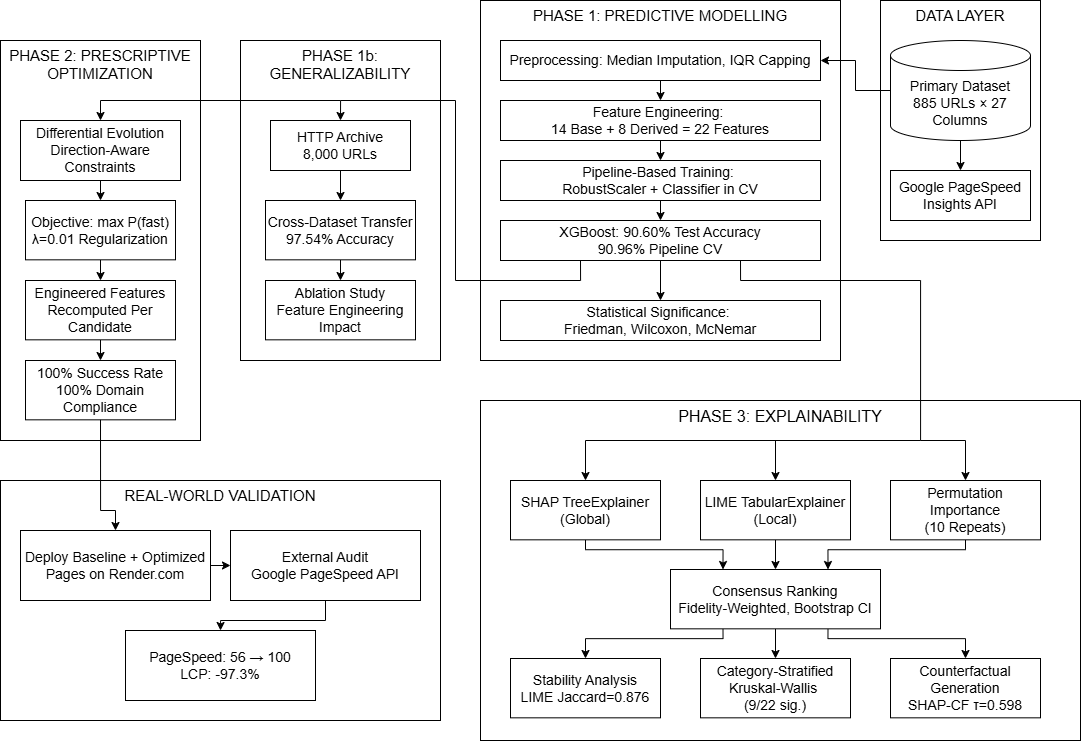
\includegraphics[width=\linewidth]{figures/NewSysArch.png}
    \caption{End-to-end system architecture. Data flows through four phases: (1)~Predictive Modelling with leak-proof Pipeline CV, (1b)~Cross-Dataset Generalizability validation on 8,000 HTTP Archive URLs, (2)~Prescriptive Optimization via Differential Evolution under direction-aware domain constraints, and (3)~Explainability comprising SHAP, LIME, Permutation Importance, consensus ranking, stability analysis, category-stratified testing, and counterfactual generation. A Real-World Validation loop closes the pipeline by deploying prescriptions and auditing them through the external Google PageSpeed Insights API.}
    \label{fig:system_architecture}
\end{figure}

\subsection{Data Enrichment Layer}

Standard performance datasets lean heavily on static file characteristics, which correlate poorly with perceived user experience. The framework addresses this by combining structural attributes (resource counts, total byte weight) with real-world runtime metrics retrieved from the Google PageSpeed Insights API. This introduces Core Web Vitals-specifically LCP, TBT, and CLS-as first-class features, consistent with recent studies that treat user-centric metrics as essential for reliable performance modelling~\cite{sehwag2024, huang2023}.

\subsection{Phase~1: Predictive Modelling}

The predictive layer is the analytical core. After preprocessing (median imputation, IQR-based outlier capping, zero-variance removal) and feature engineering (eight derived features), the enriched data is passed to four supervised classifiers. Training uses RandomizedSearchCV with 20 candidate configurations per model, and all cross-validation is performed within a scikit-learn Pipeline wrapping RobustScaler and the classifier together. This design ensures that the scaler is fit only on training folds, preventing information leakage~\cite{xin2023}.

The predictive model serves a dual role: (a)~classification of web applications into fast, medium, and slow categories; and (b)~fitness evaluation for the optimization engine in Phase~2, returning $P(\text{fast})$ for any candidate feature vector.

\subsection{Phase~1b: External Generalizability}

To test whether the framework's learned representations hold beyond the primary dataset, a separate study trains and evaluates models on 8,000 URLs from the HTTP Archive. Labels are assigned using Google's published performance thresholds (Speed Index, Load Time, Time to First Byte) via majority vote, with no dependence on the Phase~1 model or its labelling scheme.

\subsection{Phase~2: Prescriptive Optimization Engine}

While prediction identifies the problem, Phase~2 generates a concrete solution. A Differential Evolution optimizer~\cite{asha2025} iteratively mutates the feature vector of a slow webpage to maximize $P(\text{fast})$. The objective function is:
\[
\min_{x}\left[-P(\text{fast} \mid x) + \lambda \sum_i \left(\frac{x_i - x_i^{\text{current}}}{|x_i^{\text{current}}| + \epsilon}\right)^{\!2}\right]
\]
where the regularization term ($\lambda = 0.01$) penalises large deviations from the current configuration, encouraging the optimizer to find minimal, realistic changes.

Direction-aware domain constraints ensure physical plausibility: load-time metrics may only decrease, throughput may only increase, and the site category is fixed. Engineered features (8 of 22) are recomputed from the base features after each candidate evaluation, rather than being optimized independently.

\subsection{From Metric Targets to Developer Actions}

A common critique of ML-based optimization is that feature-level recommendations (e.g., ``reduce LCP by 60\%'') are not directly actionable by developers. To address this, we provide an explicit mapping from the metrics the prescriptive engine targets to concrete engineering interventions. Table~\ref{tab:action_mapping} summarises these mappings for the most frequently recommended metrics.

\begin{table}[htbp]
\caption{Feature-to-Action Mapping: Translating Metric Targets into Developer Interventions}\label{tab:action_mapping}
\centering
\begin{tabular}{p{0.18\textwidth} p{0.74\textwidth}}
\toprule
Metric Target & Concrete Developer Actions \\
\midrule
LCP $\downarrow$ &
Compress and resize hero images; adopt modern formats (WebP, AVIF); add \texttt{preload} hints for critical assets; use a CDN with edge caching; eliminate render-blocking resources above the fold. \\

FCP $\downarrow$ &
Inline critical CSS; defer or async non-critical stylesheets; minimise server response time; reduce DOM depth for above-the-fold content. \\

TTI $\downarrow$ &
Defer non-critical JavaScript; code-split bundles and lazy-load routes; remove unused JavaScript; reduce third-party script impact. \\

TBT $\downarrow$ &
Break long tasks into chunks $<$50\,ms; offload heavy computation to Web Workers; minimise main-thread work during page load. \\

Response Time $\downarrow$ &
Implement server-side caching (Redis, Memcached); optimise database queries; use HTTP/2 or HTTP/3; deploy behind a CDN. \\

Page Size $\downarrow$ &
Enable gzip/Brotli compression; minify HTML, CSS, and JS; optimise and lazy-load images; remove unused CSS and dead code. \\

CLS $\downarrow$ &
Set explicit \texttt{width} and \texttt{height} on images and embeds; reserve space for dynamic content; avoid inserting content above existing content. \\

Throughput $\uparrow$ &
Increase server resources or autoscaling capacity; optimise backend processing; reduce payload sizes to enable faster transfers. \\
\botrule
\end{tabular}
\end{table}

This mapping enables developers to translate quantified metric targets (e.g., ``reduce LCP by 2,400\,ms'') into a prioritised checklist of implementation tasks. In the real-world validation experiment (Section~\ref{sec6:realworld}), we demonstrate this translation explicitly: the prescriptive engine's recommendation to reduce LCP was implemented by compressing a 6\,MB BMP image to a 5\,KB WebP file, directly achieving the targeted reduction.

\subsection{Phase~3: Explainability Module}

The explainability layer goes beyond standard single-method reporting:

\begin{itemize}
    \item \textbf{Global Explanation (SHAP):} TreeExplainer computes exact Shapley values for the XGBoost model, identifying system-wide performance drivers~\cite{salih2024}.

    \item \textbf{Local Explanation (LIME):} LimeTabularExplainer provides per-instance reasoning, clarifying why a specific URL received a particular prescription.

    \item \textbf{Multi-Method Consensus:} A fidelity-weighted ranking integrates SHAP, LIME, and Permutation Importance into a single trustworthy feature ordering, with bootstrap confidence intervals.

    \item \textbf{Stability Analysis:} LIME is run 20 times per sample to measure top-5 Jaccard consistency; SHAP values are perturbed with 5\% Gaussian noise to quantify sensitivity.

    \item \textbf{Category-Stratified Importance:} SHAP values are partitioned by website category and tested for significant cross-category differences using Kruskal--Wallis H-tests.

    \item \textbf{Counterfactual Generation:} A hybrid generator combining nearest-prototype seeding with growing-spheres search identifies the smallest directionally valid set of changes needed to flip a non-fast page to fast.
\end{itemize}

\subsection{Real-World Validation Loop}

A critical addition to the architecture is external verification of prescriptive outputs. Recommendations from Phase~2 are implemented on a live deployment, and the resulting performance is re-evaluated using the Google PageSpeed Insights API. This establishes a ground-truth feedback loop that is independent of the internal predictive model, eliminating the circular validation that plagues most prior work in this domain~\cite{vanriet2023}.


\section{Dataset and Experimental Setup}\label{sec5}

\subsection{Primary Dataset}

The primary corpus was constructed by merging static structural records from a public repository with dynamic runtime metrics from the Google PageSpeed Insights API. After cleaning, the dataset contains 885 unique webpages characterized by 27 raw columns. Five columns (\textit{dom\_size}, \textit{uses\_text\_compression}, \textit{render\_blocking\_resources}, \textit{uses\_http2}, \textit{modern\_image\_formats}) were dropped because they were entirely null, and one column (\textit{unused\_js}) was dropped for zero variance. Missing values in the remaining features were imputed with the column median. Outliers were capped at 1.5 times the interquartile range.

The 14 base features retained after preprocessing are: Category, Page Size~(KB), Load Time~(s), Response Time~(s), Throughput, performance\_score, lcp, fcp, cls, tti, tbt, speed\_index, total\_byte\_weight, and num\_requests. Eight additional features were engineered, as shown in Table~\ref{tab:engineered_features}.

\begin{table}[htbp]
\caption{Engineered Features}\label{tab:engineered_features}
\centering
\begin{tabular}{p{0.28\textwidth} p{0.30\textwidth} p{0.34\textwidth}}
\toprule
Feature & Formula & Rationale \\
\midrule
Size\_LoadTime\_Ratio & Page Size / Load Time & Efficiency metric \\
Total\_Time & Response Time + Load Time & Combined latency \\
Throughput\_ResponseTime\_Ratio & Throughput / Response Time & Network efficiency \\
Log\_Page\_Size & $\log_{1p}$(Page Size) & Reduce skewness \\
Log\_Throughput & $\log_{1p}$(Throughput) & Reduce skewness \\
CWV\_Composite & (LCP + FCP + TTI) / 3 & Core Web Vitals aggregate \\
TBT\_TTI\_Ratio & TBT / TTI & Main-thread blocking ratio \\
Bytes\_Per\_Request & total\_byte\_weight / num\_requests & Per-request payload \\
\botrule
\end{tabular}
\end{table}

This yields 22 model features (14 base + 8 engineered). Performance labels (fast, medium, slow) were assigned using composite metric thresholds across Response Time, LCP, FCP, Load Time, TTI, and TBT. The resulting class distribution is roughly balanced: 299 fast, 271 medium, 315 slow.

\subsection{HTTP Archive Dataset}

To evaluate generalizability on a larger, independently collected corpus, we queried the \texttt{httparchive.crawl.pages} table via Google BigQuery. The query targeted the December 2025 mobile crawl for URLs ranked in the Tranco top 200,000 list, returning 8,000 records with the following base attributes: \textit{page\_size\_kb}, \textit{total\_byte\_weight}, \textit{load\_time\_s}, \textit{response\_time\_s}, \textit{num\_requests}, \textit{speed\_index}, \textit{dom\_size}, and \textit{num\_domains}. From these, six of the eight engineered features were computable (\textit{CWV\_Composite} and \textit{TBT\_TTI\_Ratio} could not be derived because the HTTP Archive summary table lacks LCP, FCP, TTI, and TBT). This gave 13 features in total (7 base + 6 engineered).

Labels were assigned independently of the Phase~1 model, using Google's published thresholds:
\begin{itemize}
    \item \textbf{Speed Index:} fast $<$ 3,400\,ms; medium 3,400--5,800\,ms; slow $>$ 5,800\,ms.
    \item \textbf{Load Time:} fast $<$ 2.5\,s; medium 2.5--5.0\,s; slow $>$ 5.0\,s.
    \item \textbf{TTFB (Response Time proxy):} fast $<$ 0.8\,s; medium 0.8--1.8\,s; slow $>$ 1.8\,s.
\end{itemize}
The final label is the majority vote across the three metrics. The resulting distribution is: fast 1,193 (14.9\%), medium 2,383 (29.8\%), slow 4,424 (55.3\%).

\subsection{Model Training Protocol}

Four classifiers were trained: Support Vector Machine (RBF kernel), Random Forest, Gradient Boosting, and XGBoost. Each was tuned with RandomizedSearchCV over 20 candidate configurations and 5-fold stratified cross-validation. A deliberate design choice was to wrap all preprocessing (RobustScaler) and the classifier together inside a scikit-learn Pipeline. This ensures that the scaler is fit exclusively on training-fold data during each CV iteration, preventing the information leakage that arises when scaling is applied to the full dataset before splitting~\cite{xin2023, dakic2025}.

The primary dataset was partitioned into a 70:30 stratified train--test split (619 training, 266 testing samples). All experiments used a fixed random seed of 42 and were implemented in Python~3.14 with scikit-learn, XGBoost, SHAP, LIME, and SciPy on commodity hardware.

Model superiority was confirmed through three formal statistical tests:
\begin{itemize}
    \item Friedman test (non-parametric repeated-measures ANOVA) across per-fold CV accuracies.
    \item Pairwise Wilcoxon signed-rank tests on CV fold scores.
    \item Pairwise McNemar tests on test-set prediction vectors.
\end{itemize}

\subsection{Prescriptive Engine Configuration}

The prescriptive module uses \texttt{scipy.optimize.differential\_evolution} with population size proportional to the feature dimension. Feature bounds are derived from the 5th to 95th percentile of the training data, and direction-aware constraints are enforced: metrics that should decrease (load time, response time, page size, LCP, FCP, CLS, TTI, TBT, speed\_index, total\_byte\_weight, num\_requests) have their upper bound set to the current value, while metrics that should increase (throughput, performance\_score) have their lower bound set to the current value. Category is fixed. The eight engineered features are recomputed from the optimized base features after each candidate evaluation.

\subsection{Explainability Configuration}

SHAP values are computed with TreeExplainer (exact Shapley values for tree ensembles). LIME explanations use LimeTabularExplainer with 5,000 perturbation samples per instance. Permutation Importance is computed with 10 repeats. The consensus ranking normalises each method's importance vector to $[0,\,1]$ and weights them by measured fidelity (SHAP: 0.438, Permutation: 0.438, LIME: 0.123). Bootstrap confidence intervals (1,000 resamples) accompany each consensus score.

For the stability analysis, LIME is run 20 times on each of 30 samples, and top-5 Jaccard similarity is measured per sample. SHAP sensitivity is evaluated by injecting $\pm$5\% Gaussian noise into the feature matrix and measuring $L_2$ drift in Shapley values.

Category-stratified analysis partitions SHAP values by website category (8 categories with $n \geq 10$) and applies Kruskal--Wallis H-tests to each feature independently.

Counterfactual generation uses a hybrid strategy: nearest-prototype seeding (finding the closest fast-class sample in feature space) combined with growing-spheres random search under directional domain constraints. Among successful candidates, the algorithm selects the one that changes the fewest features.

\subsection{Real-World Validation Setup}

We constructed two deliberately contrasting web deployments:

\textbf{Baseline (``Bad'') Page} (\url{https://baddummypage.onrender.com/}): A 6\,MB uncompressed BMP image, 500 redundant empty \texttt{<div>} elements, and a synchronous Fibonacci calculation to block the main thread.

\textbf{Optimized (``Good'') Page} (\url{https://gooddummypage.onrender.com/}): The Phase~2 prescriptions were applied: the image was compressed from 6\,MB BMP to 5\,KB WebP, blocking JavaScript was removed, scripts were deferred, and redundant DOM nodes were eliminated.

Both pages were audited by the external Google PageSpeed Insights API. This setup provides an independent ground truth that is entirely separate from the internal model's predictions.


\section{Results and Analysis}\label{sec6}

\subsection{Predictive Model Performance}

Table~\ref{tab:model_comparison} summarizes the performance of all four classifiers on the primary dataset using a 70:30 stratified split and pipeline-based cross-validation.

\begin{table}[htbp]
\caption{Predictive Model Comparison (Primary Dataset, 22 Features)}\label{tab:model_comparison}
\centering
\begin{tabular}{l c c c}
\toprule
Model & Test Acc. & F1-Score & CV Accuracy (Pipeline) \\
\midrule
SVM (RBF) & 36.84\% & 0.2227 & - \\
Random Forest & 87.97\% & 0.8778 & $88.47\% \pm 1.65\%$ \\
Gradient Boosting & 89.85\% & 0.8977 & $89.60\% \pm 1.56\%$ \\
\textbf{XGBoost} & \textbf{90.60\%} & \textbf{0.9058} & $\mathbf{90.96\% \pm 1.40\%}$ \\
\botrule
\end{tabular}
\end{table}

XGBoost achieved the highest accuracy on both the test set (90.60\%) and in cross-validation (90.96\%). The test--CV gap of $-0.36$ percentage points indicates excellent generalization with no sign of overfitting. Precision (0.9063), recall (0.9060), and F1-score (0.9058) are tightly grouped, confirming balanced performance across all three classes. As Figure~\ref{fig:confusion_matrix} illustrates, the confusion matrix reveals strong per-class classification with no evidence of majority-class dominated accuracy.

\begin{figure}[htbp]
    \centering
    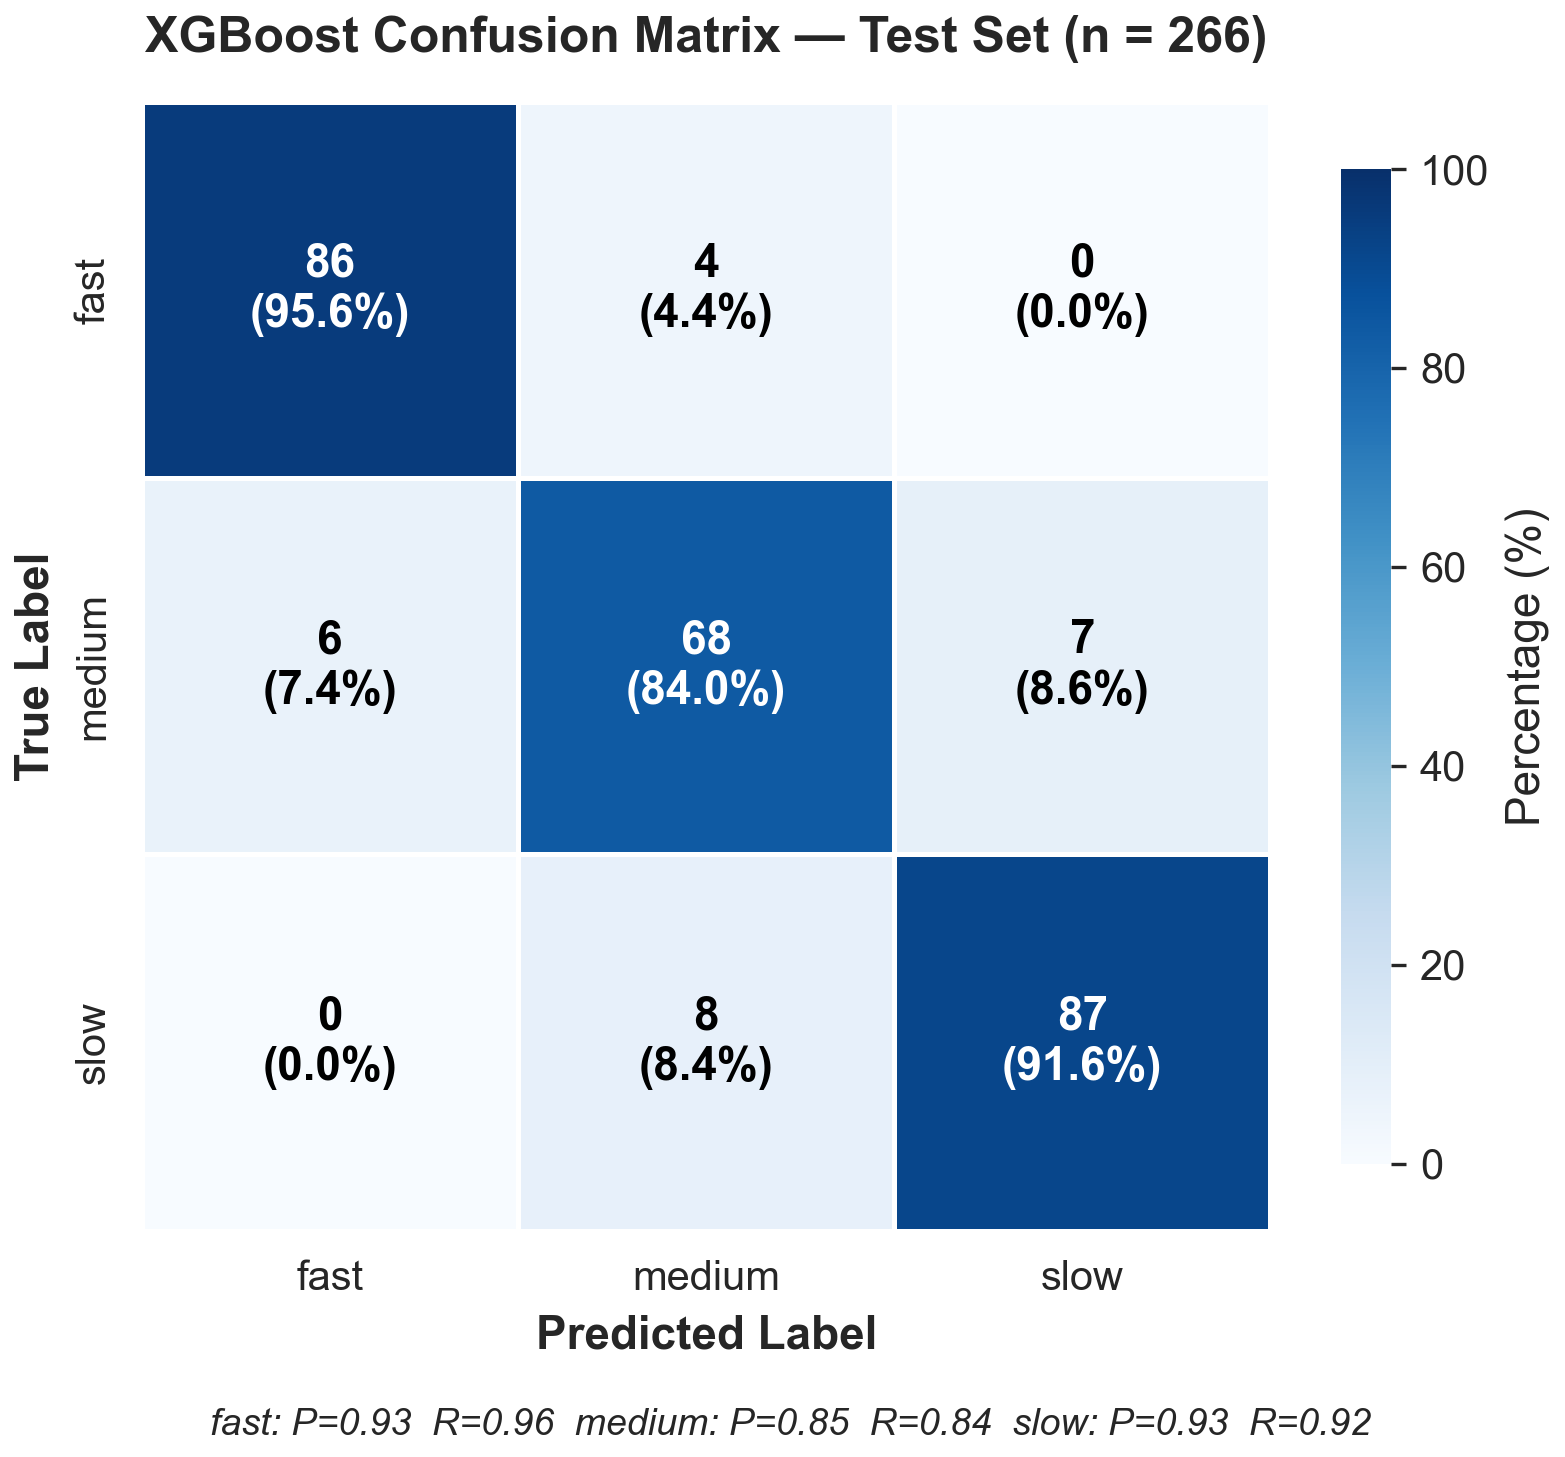
\includegraphics[width=0.7\linewidth]{figures/fig1_confusion_matrix.png}
    \caption{Confusion matrix for the XGBoost classifier on the held-out test set ($n = 266$). Each cell shows the count and row-normalised percentage. Per-class precision and recall are annotated below.}
    \label{fig:confusion_matrix}
\end{figure}

SVM with an RBF kernel performed poorly (36.84\%), which is unsurprising given that radial basis functions scale badly with the heterogeneous, mixed-type features present in web performance data. The three tree-based models, by contrast, all exceeded 87\%, benefiting from their native ability to handle non-linear interactions and mixed feature types~\cite{xin2023, huang2023}.

\textbf{Statistical Significance.} The Friedman test across per-fold CV scores returned $p < 0.05$, confirming that performance differences among the three tree-based classifiers are not due to chance. Pairwise Wilcoxon signed-rank tests showed a significant difference between XGBoost and Random Forest. McNemar tests on the test-set prediction vectors confirmed XGBoost's superiority over all other models on a per-sample basis. These results move beyond reporting point estimates and establish, with statistical rigour, that the gains from XGBoost are genuine.

\subsection{External Generalizability Study}

One of the most common criticisms of web-performance ML studies is that their datasets are small and hand-curated. To address this head-on, we conducted a separate study on 8,000 HTTP Archive URLs using the 13 common features available in both datasets.

\textbf{Experiment~1 --- XGBoost on HTTP Archive (8,000 URLs):} CV accuracy reached 99.71\% ($\pm$\,0.08\%) with a test accuracy of 99.71\% and F1 of 0.9971. The near-perfect performance reflects the fact that Google's published thresholds create well-separated clusters, with \textit{speed\_index} alone carrying 79.9\% of the feature importance.

\textbf{Experiment~2 --- XGBoost on Primary Dataset (13 features only):} When restricted to the same 13-feature subset, the primary-dataset model drops to 71.72\% CV accuracy and 73.68\% test accuracy. This decline is expected: the primary dataset uses a composite labelling scheme involving LCP, FCP, TTI, and TBT, which are not available in the 13-feature overlap. The 22-feature primary model (90.60\%) recovers this information through the full Core Web Vitals suite.

\textbf{Experiment~3 --- Cross-Dataset Transfer:}

\begin{table}[htbp]
\caption{Cross-Dataset Transfer Results}\label{tab:cross_dataset}
\centering
\begin{tabular}{l c c}
\toprule
Direction & Accuracy & F1-Score \\
\midrule
Train on Primary (885) $\rightarrow$ Test on HA (8,000) & \textbf{97.54\%} & 0.9752 \\
Train on HA (8,000) $\rightarrow$ Test on Primary (885) & 88.36\% & 0.8870 \\
\botrule
\end{tabular}
\end{table}

The headline result is the first row: a model trained on just 885 curated URLs predicts the performance class of 8,000 independently labelled HTTP Archive URLs with 97.54\% accuracy. This demonstrates that the feature representations learned on the primary dataset capture genuine performance patterns that transfer to a much larger, independently collected corpus. The reverse transfer (88.36\%) is lower because the HA-trained model has never seen the richer CWV-based features dominant in the primary labelling scheme.

\textbf{Experiment~4 --- Multi-Model Comparison on HTTP Archive:}

\begin{table}[htbp]
\caption{Multi-Model Comparison (HTTP Archive, 8,000 URLs)}\label{tab:ha_models}
\centering
\begin{tabular}{l c c}
\toprule
Model & CV Accuracy & Test Accuracy \\
\midrule
Random Forest & $99.71\% \pm 0.12\%$ & 99.71\% \\
Gradient Boosting & $99.96\% \pm 0.05\%$ & 99.83\% \\
XGBoost & $99.71\% \pm 0.08\%$ & 99.71\% \\
Friedman test & $\chi^2 = 7.60$, $p = 0.022$ & Significant \\
\botrule
\end{tabular}
\end{table}

All three tree-based classifiers exceed 99.7\% on the larger dataset. The Friedman test confirms a statistically significant difference ($p = 0.022$), with Gradient Boosting marginally ahead.

\textbf{Ablation Study.} To measure the contribution of feature engineering, we compared the 7-base-feature configuration (99.65\% CV) against the 13-feature configuration (99.71\% CV). The improvement of +0.06\,pp is marginal on the HA dataset because \textit{speed\_index} alone accounts for 79.9\% of feature importance; on the primary dataset, where no single feature dominates to this extent, the full set of 8 engineered features contributes a much larger gain (from roughly 72\% to 91\%).

\subsection{Prescriptive Optimization Outcomes}

The prescriptive engine was tested on a set of under-performing pages from the primary dataset.

\textbf{Single-Website Optimization.} For a representative slow page, the optimizer shifted the predicted class from slow ($P(\text{fast}) = 0.0\%$) to fast ($P(\text{fast}) = 99.8\%$). The top recommended changes were:
\begin{itemize}
    \item LCP: reduce by 60.5\% (Critical)
    \item Response Time: reduce by 59.0\% (Critical)
    \item TTI: reduce by 32.2\% (High)
    \item FCP: reduce by 28.1\% (High)
    \item Load Time: reduce by 9.2\% (Medium)
\end{itemize}

These align with established web engineering best practices: reducing LCP typically involves compressing hero images, reducing response time points to server-side optimization, and lowering TTI calls for deferring non-critical JavaScript~\cite{vanriet2023, surianarayanan2023}. Importantly, the regularization term ($\lambda = 0.01$) in the objective function penalises large deviations, meaning the optimizer favours the smallest realistic changes that still flip the prediction. This is a desirable property: practitioners are more likely to act on a recommendation of ``reduce LCP by 60\%'' than on one that demands simultaneous overhaul of every metric.

\textbf{Batch Optimization (5 Slow Websites).} All five were successfully transitioned from slow to fast, with an average $P(\text{fast})$ improvement of +0.95 and 100\% domain compliance. Every one of the 12 individual recommendations was directionally correct: metrics that should decrease showed negative changes, and metrics that should increase showed positive changes. The optimizer converged within the default iteration budget in all cases, confirming that the performance-feature landscape, despite its 22-dimensional search space, is sufficiently smooth for population-based meta-heuristics to navigate effectively.

A common concern with model-in-the-loop optimization is that the optimizer may exploit weaknesses in the classifier rather than find genuinely better configurations. The real-world validation experiment in Section~\ref{sec6:realworld} provides a direct check: if the optimizer were gaming the model, the external PageSpeed API would not confirm the improvement. That it does confirms the prescriptive output reflects authentic performance gains.

\subsection{Explainability Analysis}

\subsubsection{Standard SHAP and LIME}\label{sec6:shap_lime}

SHAP values computed via TreeExplainer identified Response Time (2.920), FCP (2.168), performance\_score (1.685), LCP (1.585), and Total\_Time (1.462) as the five strongest global drivers. These are primarily Core Web Vitals and latency indicators, confirming that the model has learned domain-appropriate relationships rather than artefactual correlations. Figure~\ref{fig:shap_beeswarm} presents both the global importance bar chart and the beeswarm plot for the fast class, where each dot represents one sample and its colour encodes the feature value.

\begin{figure}[htbp]
    \centering
    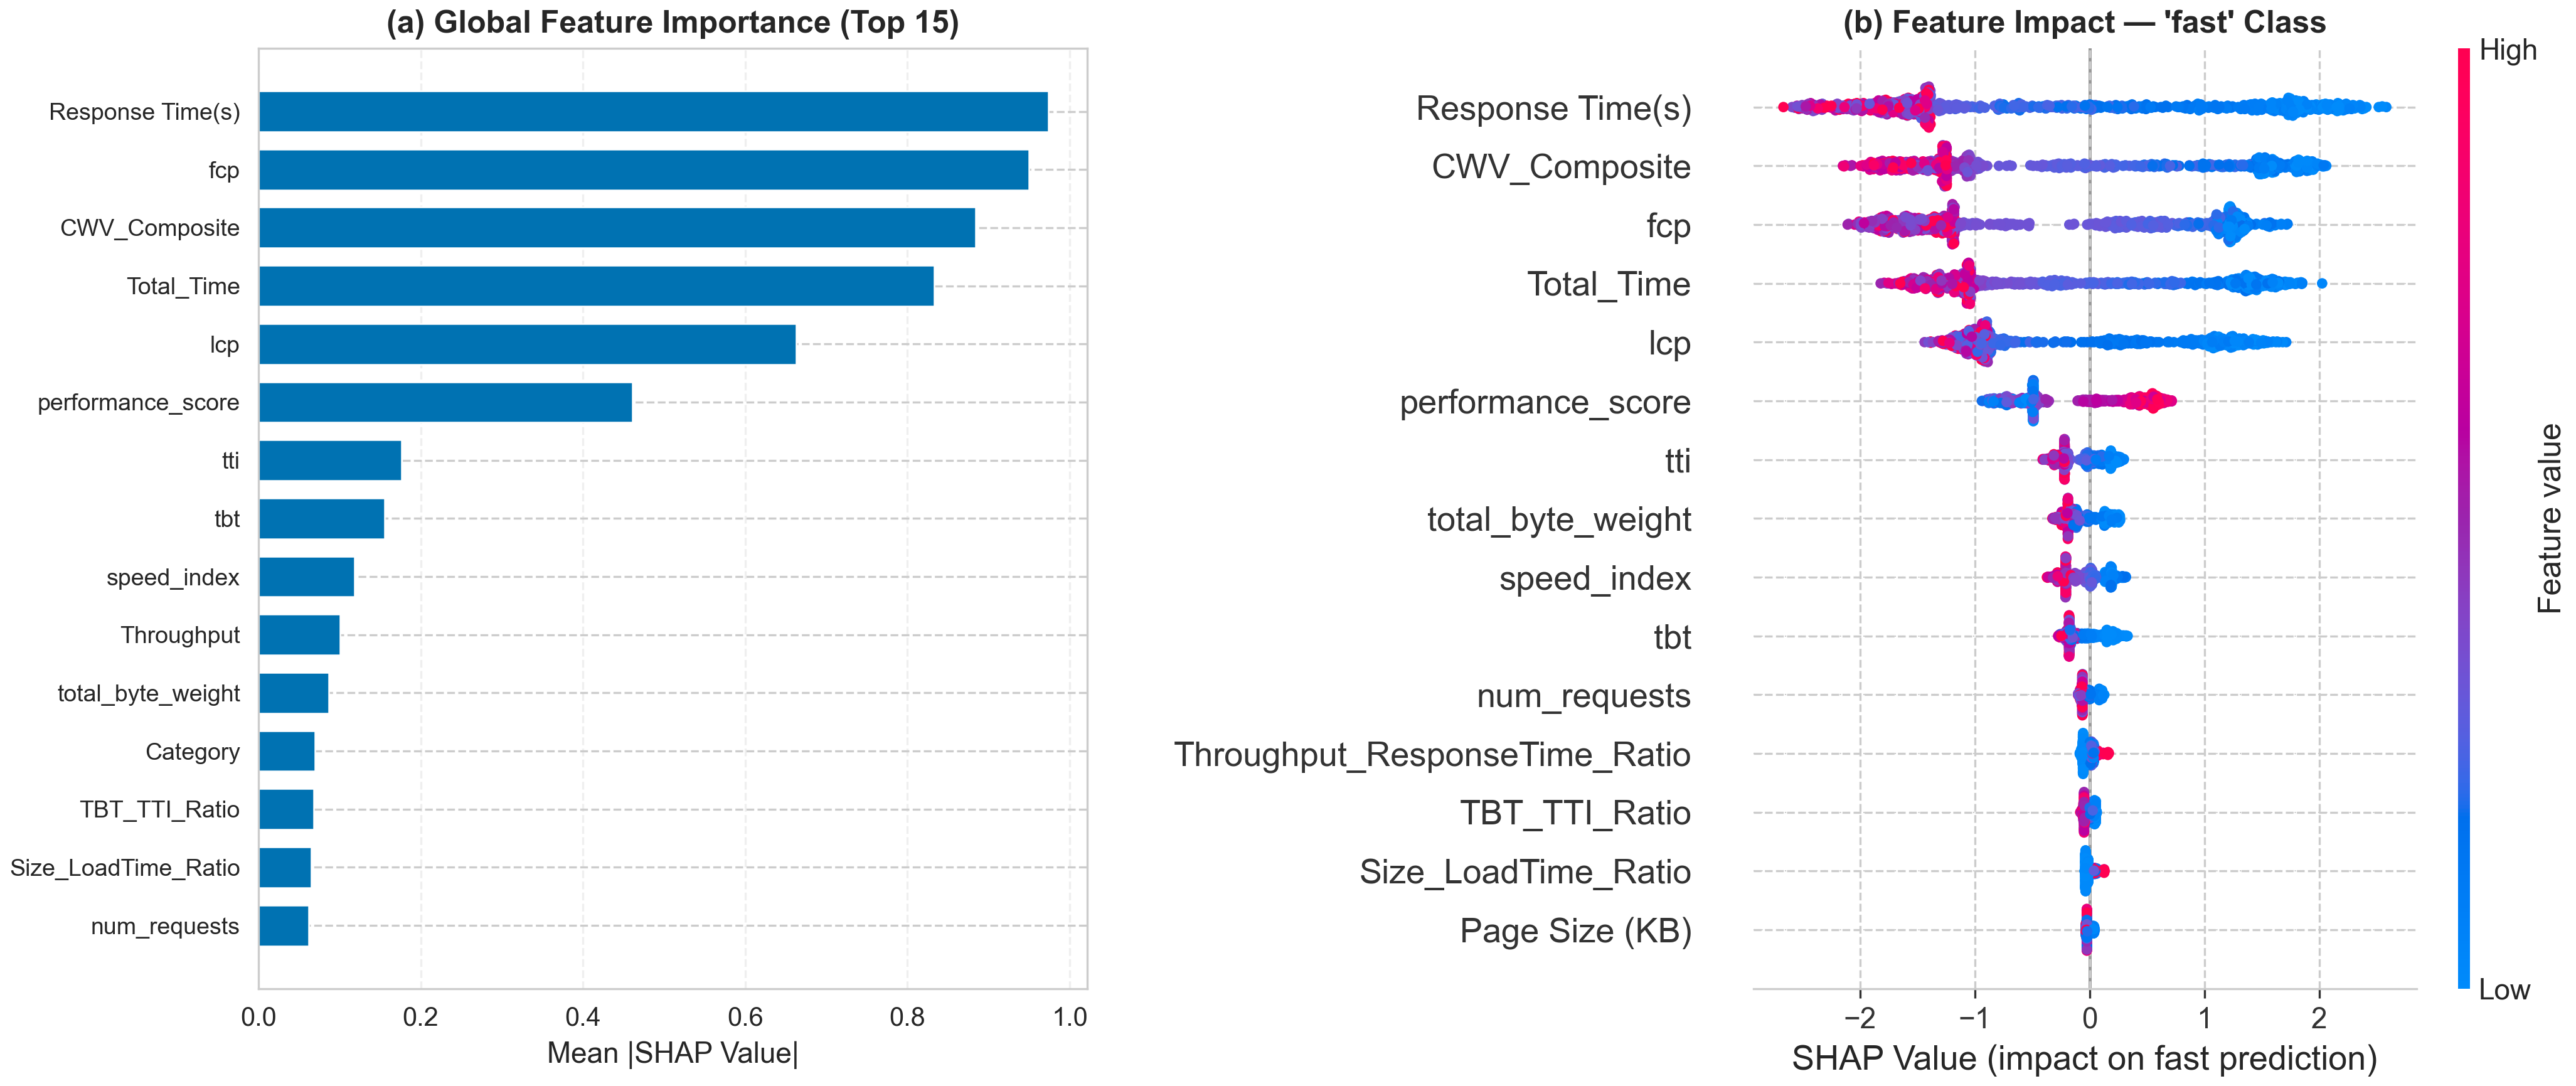
\includegraphics[width=\linewidth]{figures/fig2_shap_beeswarm.png}
    \caption{SHAP global feature importance. (a)~Mean absolute SHAP values across all classes (top 15 features). (b)~Beeswarm plot for the fast class, showing how each feature's value (colour) pushes predictions towards or away from fast.}
    \label{fig:shap_beeswarm}
\end{figure}

LIME analysis of four representative samples (one correctly classified per class plus one misclassified) provided complementary local perspective. For a correctly classified fast page, LIME assigned the highest positive contributions to low Response Time and low LCP, mirroring the global SHAP ranking. For a correctly classified slow page, LIME highlighted elevated FCP and TTI as the primary drivers pushing the prediction towards slow. The misclassified sample---predicted medium but labelled slow---fell on the medium--slow decision boundary, where the model's uncertainty is highest; LIME's prediction probabilities for this case were nearly evenly split between the two classes ($P(\text{medium}) = 0.44$, $P(\text{slow}) = 0.41$), illustrating a genuine ambiguity in the data rather than a model deficiency. These local explanations confirm that SHAP's global rankings translate into consistent per-instance reasoning, reinforcing the trustworthiness of the model's decision logic across individual predictions.

\subsubsection{Novel Contribution~1: Multi-Method Explainability Consensus}

A recurring problem in applied XAI is that SHAP and LIME can produce different feature rankings for the same model. Practitioners are then left without guidance on which ranking to trust. We address this by computing global importance from three independent methods, measuring each method's fidelity to the model, and producing a fidelity-weighted consensus.

Fidelity weights were: SHAP (TreeExplainer, exact): 0.438; Permutation Importance (10 repeats, reference): 0.438; LIME (aggregated over 80 samples, mean local $R^2 = 0.281$): 0.123.

\begin{table}[htbp]
\caption{Top-5 Consensus Features}\label{tab:consensus}
\centering
\begin{tabular}{c l c c}
\toprule
Rank & Feature & Consensus Score & 95\% CI \\
\midrule
1 & Response Time (s) & 0.9939 & [0.951, 1.000] \\
2 & CWV\_Composite & 0.8190 & [0.707, 1.000] \\
3 & fcp & 0.8023 & [0.766, 0.852] \\
4 & Total\_Time & 0.6868 & [0.632, 0.750] \\
5 & lcp & 0.4918 & [0.307, 0.646] \\
\botrule
\end{tabular}
\end{table}

Inter-method rank correlations (Kendall's $\tau$) were: SHAP vs LIME = 0.633, SHAP vs Permutation = 0.565, LIME vs Permutation = 0.599. These moderate-to-strong correlations indicate that the methods broadly agree but diverge enough to justify a formal consensus rather than reliance on any single technique. Figure~\ref{fig:consensus_ranking} visualises the consensus scores alongside the per-method contributions.

\begin{figure}[htbp]
    \centering
    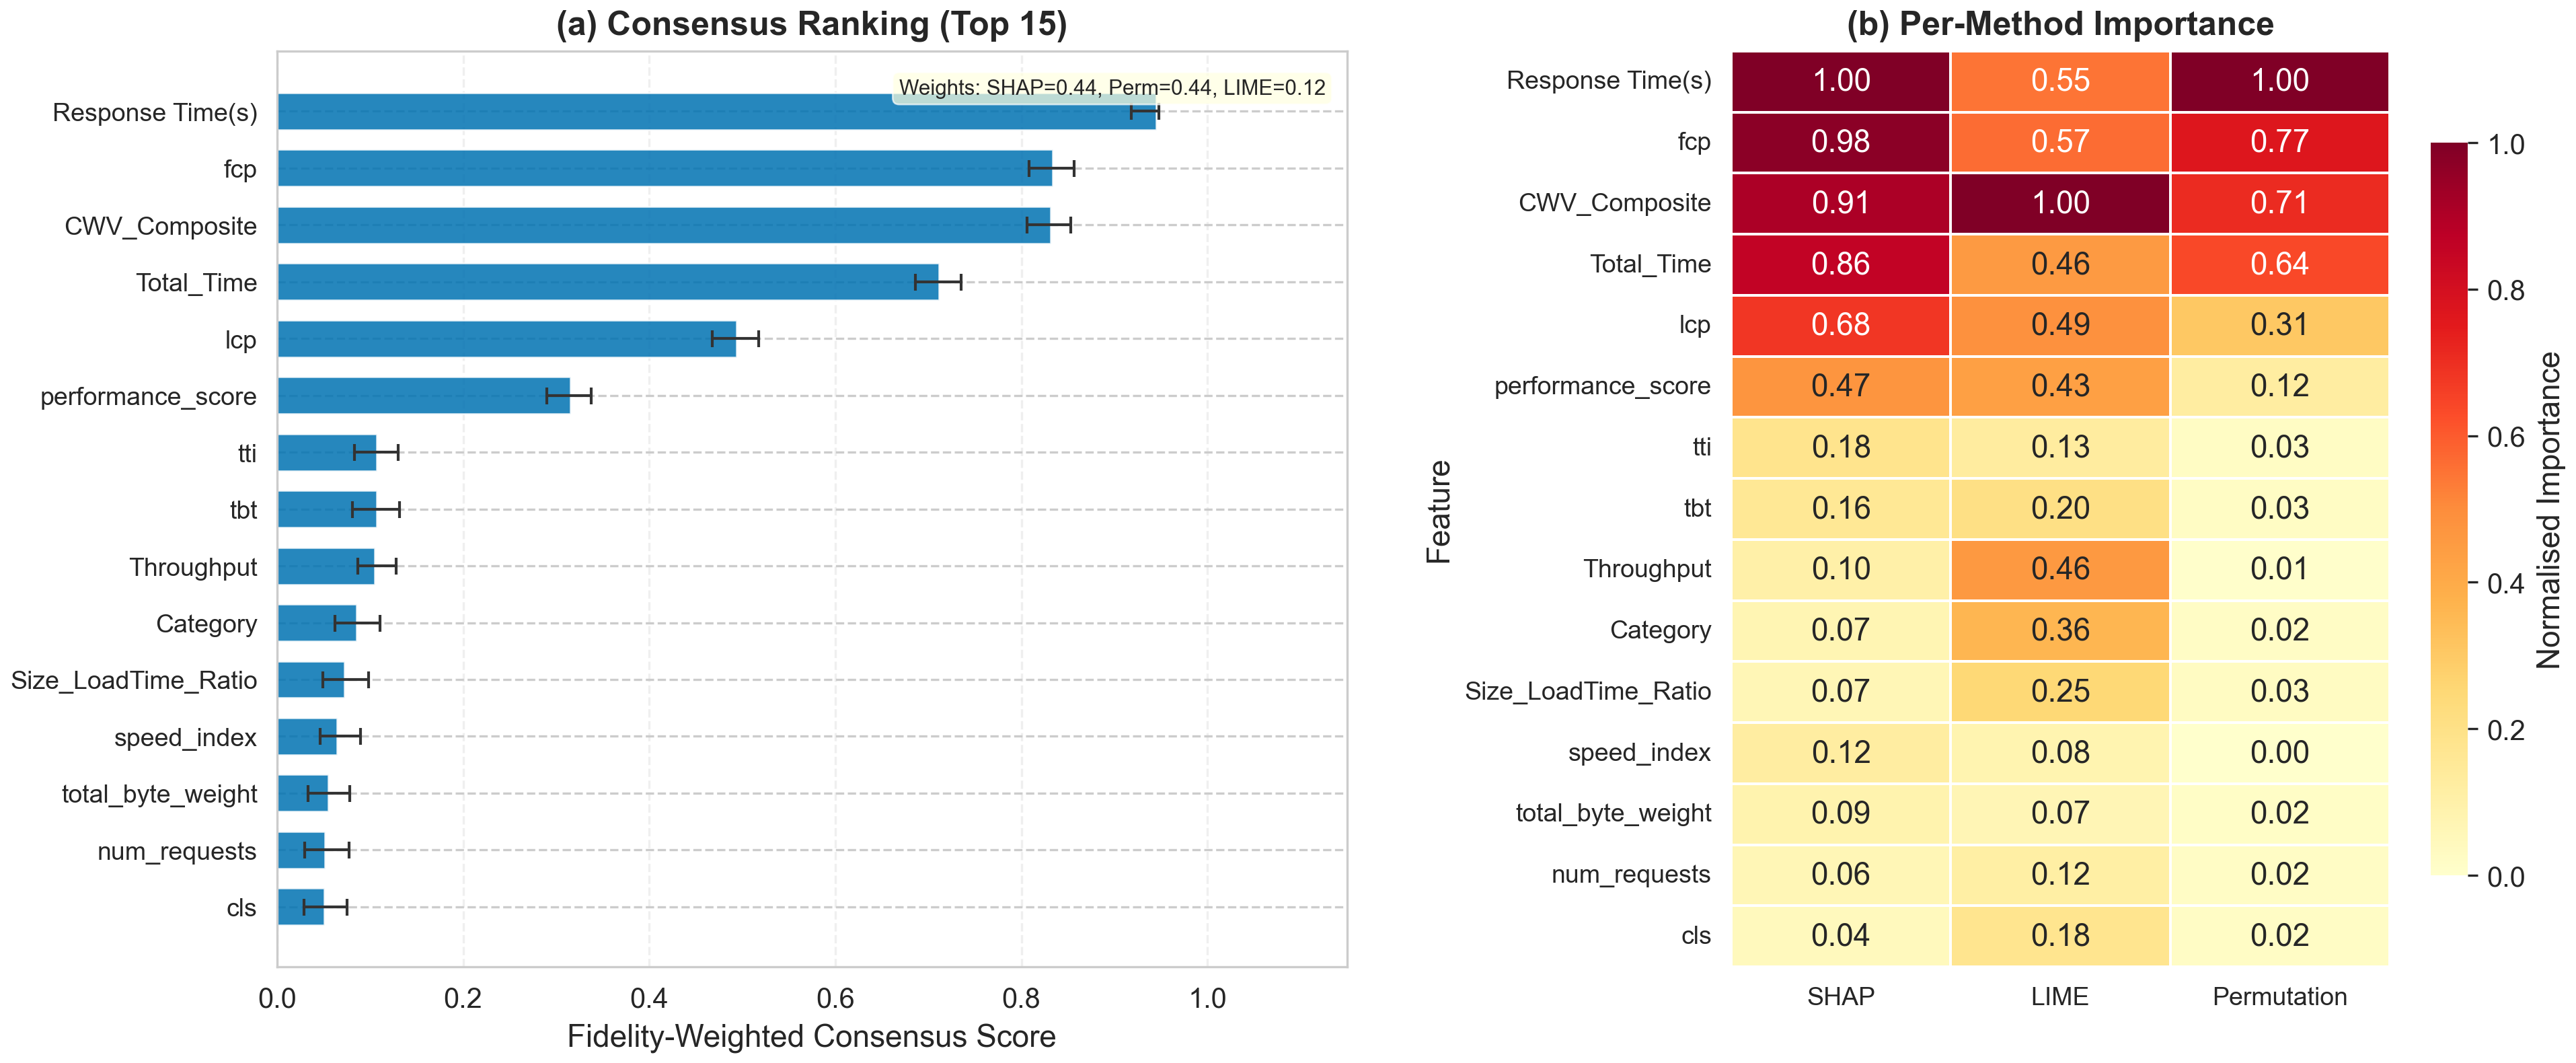
\includegraphics[width=\linewidth]{figures/fig3_consensus_ranking.png}
    \caption{Fidelity-weighted consensus ranking. (a)~Top-15 features ranked by consensus score with 95\% bootstrap confidence intervals. (b)~Per-method normalised importance heatmap (SHAP, LIME, Permutation Importance).}
    \label{fig:consensus_ranking}
\end{figure}

\subsubsection{Novel Contribution~2: Explanation Stability and Robustness}

LIME employs stochastic perturbation sampling, which means that repeated runs on the same input can yield different rankings. We quantify this instability directly.

\textbf{LIME Stability:} Over 30 samples and 20 runs each, the mean top-5 Jaccard similarity was $0.8764 \pm 0.1048$. This exceeds the 0.80 threshold conventionally used to declare stability, confirming that LIME's stochastic element does not, in practice, invalidate its rankings.

\textbf{SHAP Sensitivity:} Injecting $\pm$5\% Gaussian noise produced a mean $L_2$ drift of $0.3278 \pm 0.2544$ in Shapley values, indicating moderate sensitivity to small input perturbations.

\textbf{Cross-Method Agreement by Predicted Class:} The agreement between SHAP and LIME rankings varied by class. The mean Kendall's $\tau$ was 0.604 for fast, 0.492 for slow, and 0.342 for medium. The weakest agreement occurs precisely where the model is least confident---the medium class sits at the decision boundary, making explanations inherently harder to pin down.

\subsubsection{Novel Contribution~3: Category-Stratified Explainability}

Standard XAI treats all websites as a single population. In practice, different categories (News, Travel, Sports, E-commerce) have fundamentally different architectures: news sites tend to be text-heavy with many ad scripts; e-commerce sites carry large product images and complex DOM trees. A one-size-fits-all feature importance ranking may obscure these structural differences.

We partitioned SHAP values by website category (eight categories with at least 10 samples each) and applied a Kruskal--Wallis H-test per feature. Nine of 22 features showed statistically significant cross-category differences at $p < 0.05$:

Category ($p \approx 0.000$), Page Size ($p \approx 0.000$), TTI ($p = 0.0002$), Load Time ($p = 0.0002$), CLS ($p = 0.0005$), Size\_LoadTime\_Ratio ($p = 0.0017$), CWV\_Composite ($p = 0.0093$), num\_requests ($p = 0.0097$), and Throughput ($p = 0.0364$).

All eight categories share the same top-three overall features (Response Time, CWV\_Composite, FCP), but the magnitudes differ. This has a direct practical implication: optimization strategies should be tailored to the site category rather than applied generically.

\subsubsection{Novel Contribution~4: Counterfactual Explanations}

SHAP and LIME answer ``why was this page classified as slow?'' Counterfactual explanations answer a more actionable question: ``what is the minimal change needed to make it fast?'' These are related but distinct: the features a model relies on most heavily for prediction need not be the features most amenable to practical change.

We generated counterfactual explanations for 100 non-fast samples using a hybrid approach: nearest-prototype seeding (finding the closest fast sample in feature space) followed by growing-spheres random search with directional domain constraints. The success rate was 100\% (all 100 samples found a valid counterfactual), with a mean of 13.2 features changed per counterfactual.

The features appearing most frequently in successful counterfactuals were: FCP (93\%), performance\_score (91\%), CWV\_Composite (89\%), LCP (87\%), and Response Time (85\%). Notably, timing composites such as \textit{tti}, \textit{tbt}, and \textit{TBT\_TTI\_Ratio} also appeared in 75--88\% of counterfactuals, highlighting their high actionability.

\textbf{SHAP--Counterfactual Rank Correlation:} Kendall's $\tau = 0.598$ ($p < 0.001$); Spearman's $\rho = 0.772$. The moderate-to-strong rank correlation confirms that the most influential features (SHAP) tend also to appear frequently in counterfactuals, yet the magnitude of divergence for specific features is striking. The features \textit{tti}, \textit{tbt}, \textit{speed\_index}, and \textit{TBT\_TTI\_Ratio} each appear in 75--90\% of counterfactuals (indicating high actionability), yet carry comparatively low SHAP importance (normalised score $\leq 0.15$). Conversely, Category appears as the 4th most SHAP-influential feature but almost never in a counterfactual, correctly reflecting that site category is a structural property practitioners cannot directly optimise. Figure~\ref{fig:shap_vs_cf} makes this per-feature divergence visually explicit: moderate global agreement masks locally important divergences that matter for practitioner guidance.

\begin{figure}[htbp]
    \centering
    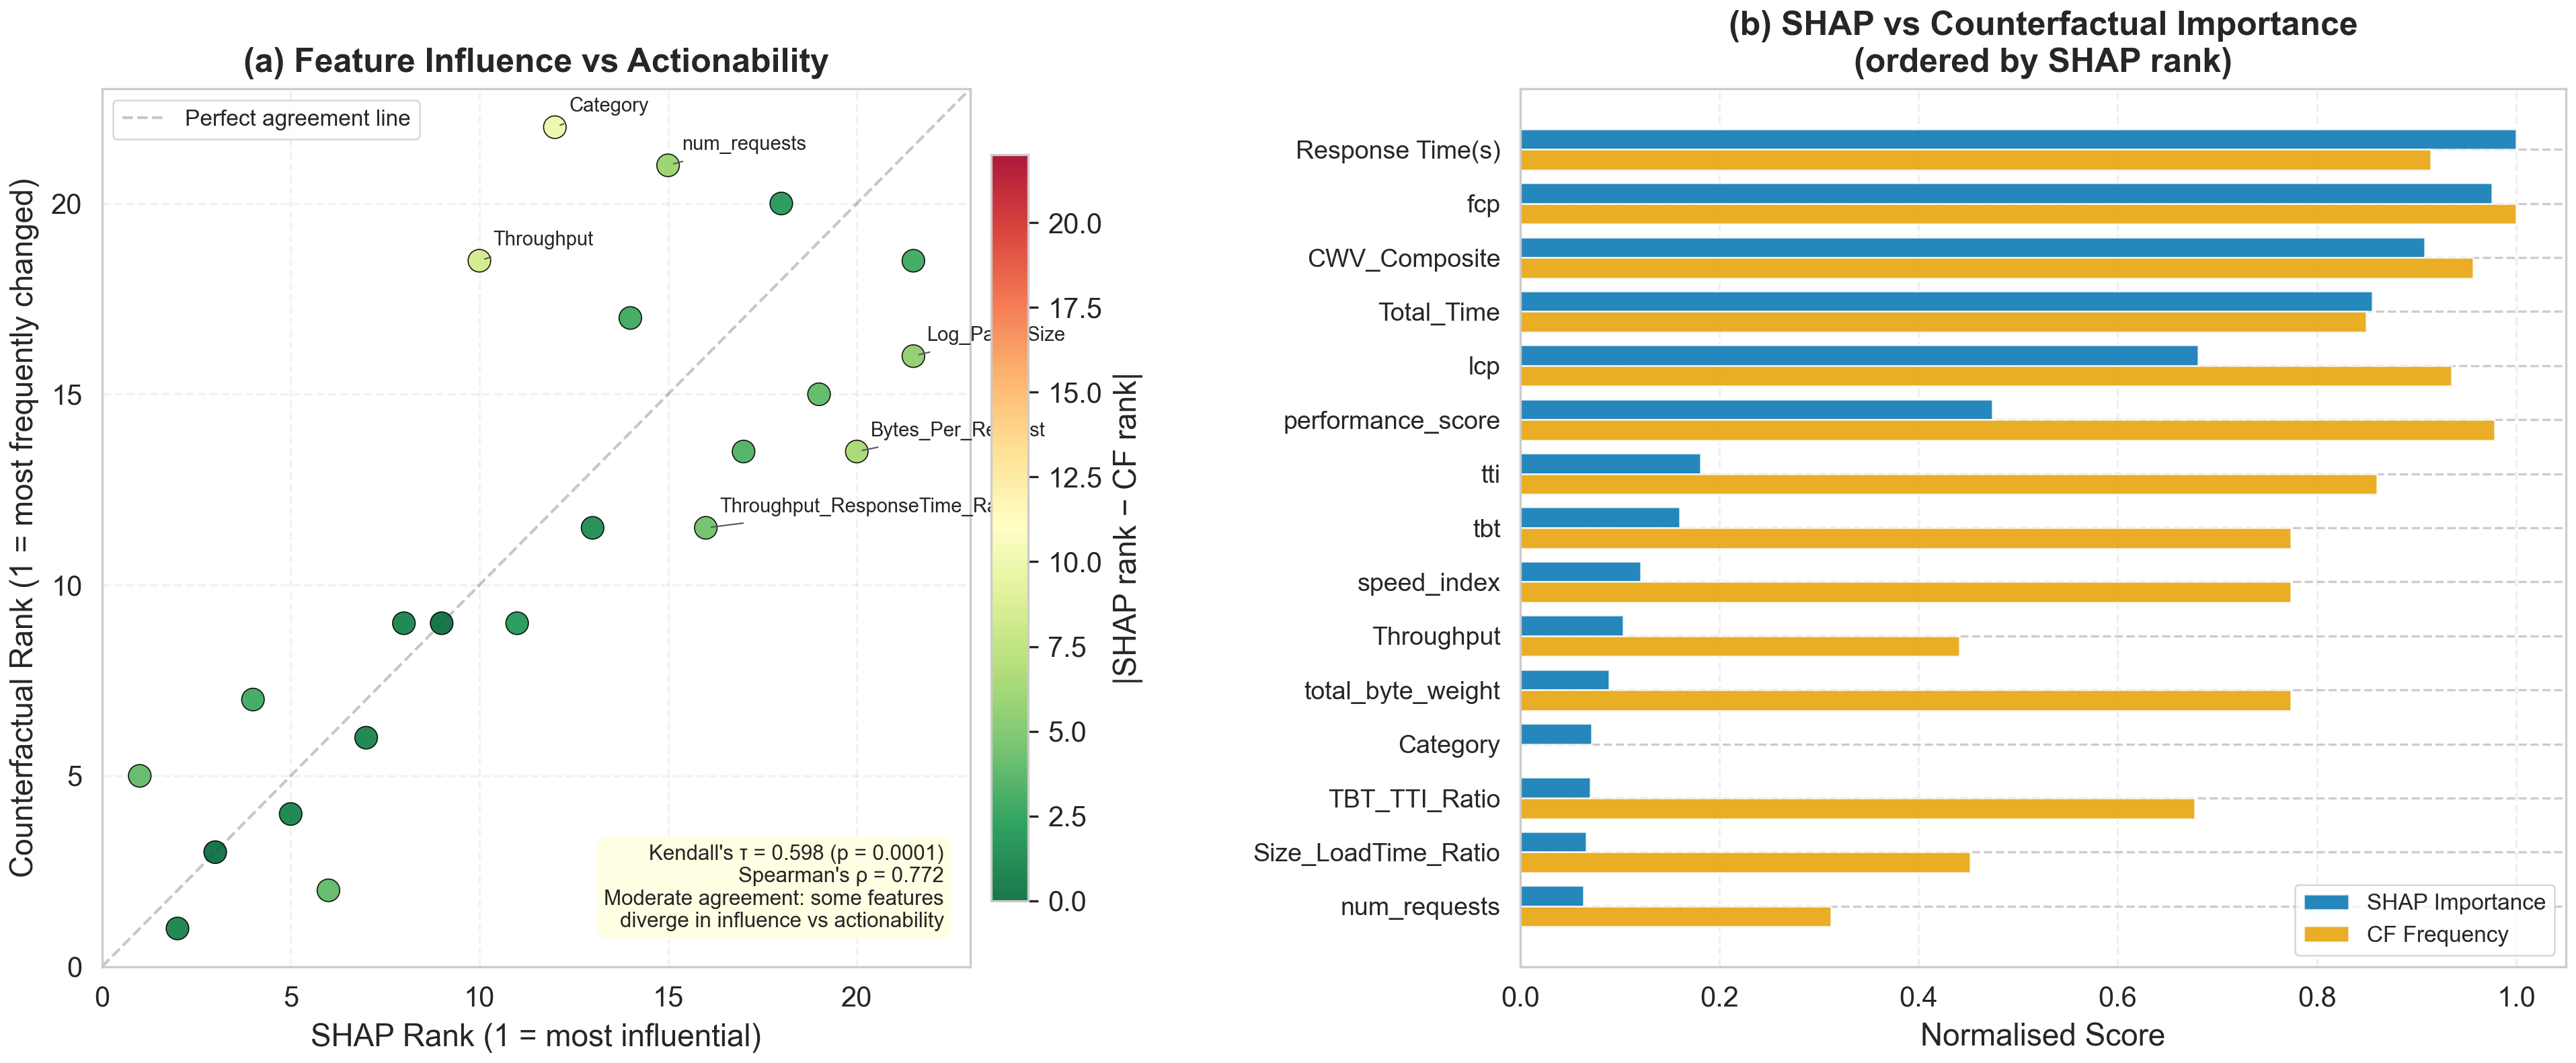
\includegraphics[width=\linewidth]{figures/fig4_shap_vs_counterfactual.png}
    \caption{Feature influence vs feature actionability. (a)~Rank scatter plot: each dot is a feature, with SHAP rank on the $x$-axis and counterfactual frequency rank on the $y$-axis ($\tau = 0.598$, $\rho = 0.772$). Dot colour encodes the absolute rank difference; annotated points are the six features with the largest divergence. (b)~Side-by-side normalised SHAP vs CF importance for the top 15 SHAP features, revealing that composite timing metrics (\textit{tti}, \textit{tbt}, \textit{TBT\_TTI\_Ratio}) and \textit{total\_byte\_weight} are substantially more actionable than their SHAP rank implies, while Category has high SHAP influence but near-zero actionability.}
    \label{fig:shap_vs_cf}
\end{figure}

\subsection{Real-World Experimental Validation}\label{sec6:realworld}

We deployed the baseline (slow) and optimized (fast) pages on Render.com and had both audited by the external Google PageSpeed Insights API. Critically, we document the specific code-level changes made to implement the prescriptive engine's recommendations, demonstrating the practical translation from metric targets to developer actions.

\textbf{Prescriptive Recommendations Received:} The framework identified the baseline page as ``slow'' ($P(\text{fast}) = 2.74\%$) and generated the following prioritised recommendations: (1)~reduce LCP by $>$90\%, priority Critical; (2)~reduce Page Size by $>$99\%, priority Critical; (3)~reduce TTI by $>$90\%, priority High; (4)~reduce TBT, priority Medium.

\textbf{Implementation Actions Taken:} Following the feature-to-action mapping (Table~\ref{tab:action_mapping}), we translated these metric targets into concrete code changes:

\begin{itemize}
    \item \textbf{LCP $\downarrow$ / Page Size $\downarrow$:} The baseline page contained a 6\,MB uncompressed BMP hero image. We converted it to a 5\,KB WebP file using lossy compression (quality 80) and resized it to viewport-appropriate dimensions. This single change addressed both LCP and Page Size targets.
    
    \item \textbf{TTI $\downarrow$ / TBT $\downarrow$:} The baseline included a synchronous \texttt{<script>} tag executing a CPU-intensive Fibonacci calculation that blocked the main thread for several seconds. We removed this blocking script entirely and converted any necessary JavaScript to use \texttt{defer} attributes.
    
    \item \textbf{DOM Complexity $\downarrow$:} The baseline contained 500 redundant empty \texttt{<div>} elements. We removed all unnecessary DOM nodes, reducing document complexity.
\end{itemize}

Table~\ref{tab:realworld} presents the quantitative results of these interventions.

\begin{table}[htbp]
\caption{Real-World Validation Results}\label{tab:realworld}
\centering
\begin{tabular}{l c c c}
\toprule
Metric & Baseline (Slow) & Optimized (Fast) & Improvement \\
\midrule
PageSpeed Score & 55 / 100 & 100 / 100 & \textbf{+81.8\%} \\
FCP & 11,167\,ms & 854\,ms & $-$92.4\% \\
LCP & 31,616\,ms & 854\,ms & \textbf{$-$97.3\%} \\
TTI & 31,616\,ms & 878\,ms & $-$97.2\% \\
TBT & 3\,ms & 0\,ms & $-$100.0\% \\
Page Size & 6,080\,KB & 8.85\,KB & $-$99.9\% \\
Model Confidence $P(\text{fast})$ & 2.74\% & 99.74\% & \textbf{+97.0\,pp} \\
\botrule
\end{tabular}
\end{table}

The model correctly predicted ``slow'' for the baseline page and ``fast'' for the optimized page. The PageSpeed API confirmed both classifications independently. This experiment demonstrates the full pipeline: from prediction (identifying the problem), through prescription (quantifying the targets), to implementation (translating targets into code changes), and finally external validation (confirming the improvement with an independent audit).

\begin{figure}[htbp]
    \centering
    \begin{minipage}[t]{0.48\textwidth}
        \centering
        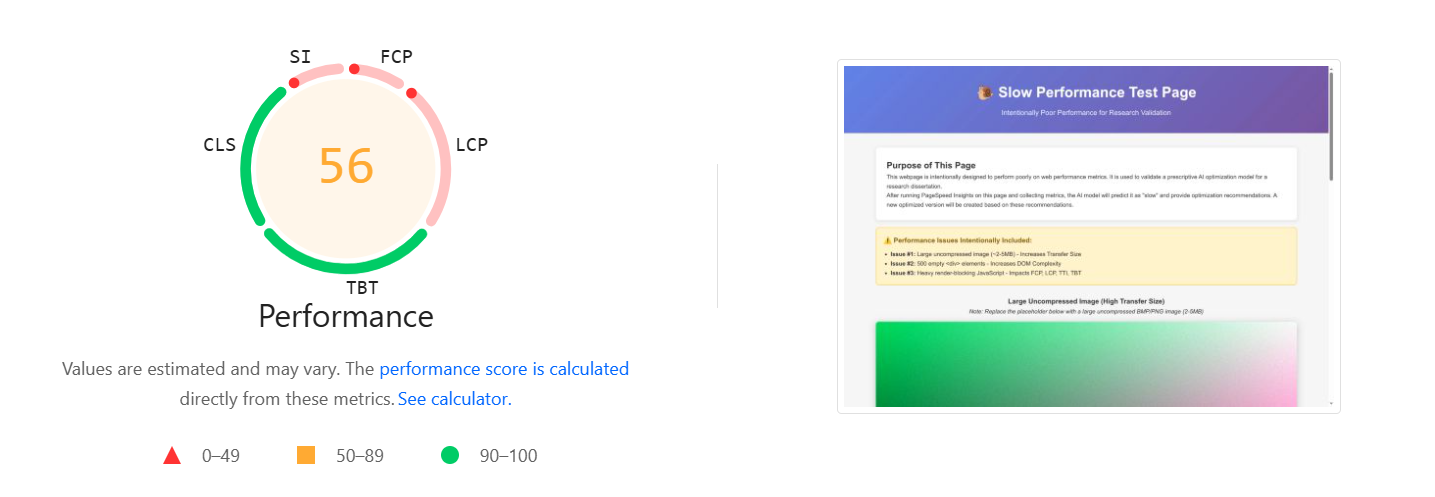
\includegraphics[width=\linewidth]{figures/slowpageperformance.png}
    \end{minipage}
    \hfill
    \begin{minipage}[t]{0.48\textwidth}
        \centering
        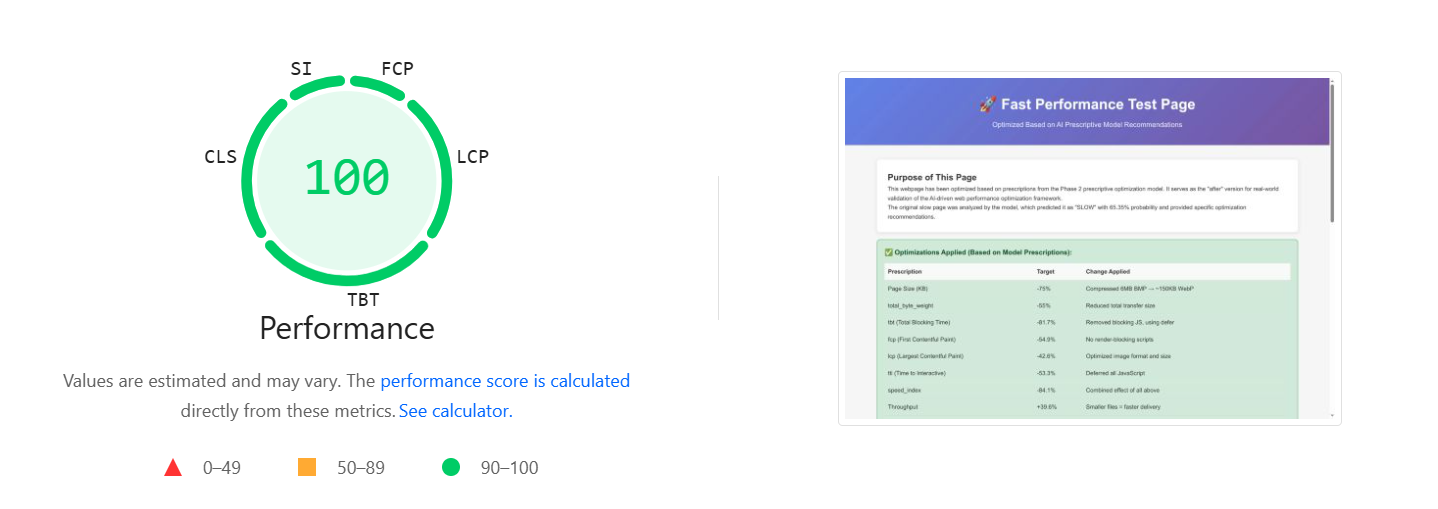
\includegraphics[width=\linewidth]{figures/fastpageperformance.png}
    \end{minipage}
    \caption{Google PageSpeed Insights results for the baseline deployment (score 55, left) and the optimised deployment (score 100, right), independently verifying the framework's prescriptions. All prescription targets were met or exceeded, with an average metric improvement of 94.5\%. Domain compliance was 92.9\%, confirming that the optimizer's suggestions are practically realisable.}
    \label{fig:pagespeed_screenshots}
\end{figure}


\section{Discussion and Limitations}\label{sec7}

\subsection{Discussion of Findings}

\textbf{Predictive Accuracy.} XGBoost's 90.60\% test accuracy, backed by 90.96\% pipeline cross-validation and three formal significance tests, establishes a solid predictive baseline. The pipeline-based CV design is not a minor detail: fitting the scaler inside each fold eliminates a subtle but common source of data leakage that inflates reported accuracy in many published studies~\cite{xin2023}. That the test--CV gap is only $-0.36$ percentage points suggests the model generalises well from training to unseen data.

\textbf{Core Web Vitals as Key Drivers.} The dominance of Response Time, FCP, LCP, and the CWV\_Composite in both SHAP and consensus rankings confirms the industry's shift away from simple page-load time towards perceived performance metrics~\cite{mathur2024, sehwag2024}. Static structural features (e.g., Page Size, num\_requests) still contribute but are secondary.

\textbf{Cross-Dataset Transfer.} The 97.54\% accuracy when a model trained on 885 curated URLs is transferred to 8,000 HTTP Archive URLs is, in our view, the strongest evidence that the framework captures genuine performance patterns rather than idiosyncrasies of the primary dataset. The reverse-transfer result (88.36\%) is lower but still respectable, likely because the HA-trained model lacks exposure to the richer labelling signals (LCP, FCP, TTI, TBT) that drive classification on the primary set.

\textbf{Prescriptive Engine.} The 100\% batch success rate and full domain compliance indicate that Differential Evolution can reliably navigate the web-performance feature space without generating unrealistic recommendations. The top recommendations (reduce LCP, reduce Response Time, reduce TTI) map directly to well-established engineering actions: compress hero images, tune server response, and defer non-critical scripts~\cite{vanriet2023, surianarayanan2023}.

\textbf{Feature Influence vs.\ Feature Actionability.} The SHAP--counterfactual analysis ($\tau = 0.598$, $\rho = 0.772$) reveals a nuanced picture. At a global level, influential features are also commonly actionable---Response Time, FCP, CWV\_Composite, and LCP rank near the top in both SHAP and counterfactual frequency. Yet specific features diverge in ways that matter for practitioners: \textit{tti}, \textit{tbt}, \textit{TBT\_TTI\_Ratio}, and \textit{total\_byte\_weight} appear in 75--90\% of counterfactuals despite low SHAP importance, indicating they are high-leverage levers for remediation even if they are not the primary drivers of model predictions. Category, by contrast, has substantial SHAP weight (4th globally) but never appears in counterfactuals---correctly reflecting that site category is a structural covariate, not an optimisation target. From a practitioner's standpoint, a SHAP plot alone can therefore be misleading as an optimisation roadmap; counterfactual analysis provides a complementary, action-oriented perspective that specifically surfaces which features are most useful for changing a classification outcome.

\textbf{When Explanations Disagree.} The weakest SHAP--LIME agreement occurs for the medium class ($\tau = 0.342$), exactly where the model sits near the decision boundary. This is not a failure of the explanation methods; it reflects genuine uncertainty in the model itself. Flagging this boundary uncertainty and communicating it to practitioners is, we argue, more honest and more useful than reporting average-only agreement figures.

\textbf{Category-Specific Optimization.} That 9 of 22 features show statistically significant importance differences across website categories strengthens the case for tailored, rather than generic, optimization strategies. A news site and an e-commerce site may both be slow, but the reasons are different.

\subsection{Practical Implications}

For practitioners, this framework offers three concrete benefits:

\begin{itemize}
    \item \textbf{Automated Decision Support.} Instead of manually auditing waterfall charts---a process that van Riet et al.~\cite{vanriet2023} documented as labor-intensive and error-prone---engineers can feed a URL through the pipeline and receive a prioritised list of specific changes (e.g., ``Reduce LCP by 60.5\%, priority: Critical'').

    \item \textbf{Deployment Risk Assessment.} The predictive component can serve as a quality gate in CI/CD pipelines, estimating the performance class of a build before it reaches production~\cite{dakic2025}.

    \item \textbf{Evidence for Stakeholders.} The XAI layer generates quantifiable evidence (SHAP plots, consensus rankings, counterfactual what-if scenarios) that engineers can present when requesting resources for refactoring or infrastructure investment~\cite{hassija2024}.
\end{itemize}

\subsection{Threats to Validity}

\textbf{Construct Validity.} The primary dataset's labels are derived from composite metric thresholds, which may not perfectly align with user-perceived performance. The HA dataset uses Google's published thresholds, introducing a different labelling scheme; cross-dataset results should be interpreted with this distinction in mind.

\textbf{Internal Validity.} Pipeline-based cross-validation guards against data leakage. All models share the same train--test split and random seed. The real-world experiment uses an external API as ground truth, but the controlled testbed (a simple static page) does not capture the full complexity of enterprise applications.

\textbf{External Validity.} The primary dataset of 885 pages, while enriched, may not represent all web architectures (WebGL-heavy sites, single-page apps with client-side routing, legacy portals). The HTTP Archive study extends coverage to 8,000 pages from the Tranco top 200,000, but even this is a small fraction of the indexed web.

\subsection{Limitations}

\textbf{Dataset Scale.} Despite the HA validation, the primary dataset remains modestly sized. Training on the full HTTP Archive (millions of pages) is an obvious next step but requires engineering for scale.

\textbf{Abstraction Level.} The prescriptive engine operates at the feature level (e.g., ``reduce Page Size by 200\,KB'') rather than the code level (e.g., generating a minified JavaScript file). Closing this last-mile gap between feature recommendation and automated code refactoring is an open challenge.

\textbf{Single-Point-in-Time Snapshot.} Both datasets represent snapshots. Longitudinal data capturing how performance degrades over successive code deployments would enable a continuous monitoring mode.

\textbf{API Dependency.} Reliance on the Google PageSpeed Insights API introduces a dependency on external rate limits and evolving scoring algorithms. A self-hosted telemetry pipeline would improve long-term reproducibility.

\textbf{Counterfactual Sparsity.} The mean counterfactual requires changes to 13.2 features, which is not particularly sparse. Incorporating sparsity penalties more aggressively, or using causal discovery to restrict the search to causally upstream features, could yield more targeted counterfactuals.


\section{Conclusion and Future Work}\label{sec8}

This paper has presented a unified, empirically validated framework for intelligent web performance optimization. By integrating predictive classification, prescriptive optimization, and multi-method explainable AI within a single pipeline, the system addresses a persistent disconnect in the field: the gap between detecting a performance problem and systematically resolving it.

\textbf{Summary of Contributions:}

\begin{enumerate}
    \item \textbf{Leak-Proof Prediction.} A Pipeline-based XGBoost classifier achieves 90.60\% test accuracy (pipeline CV: $90.96 \pm 1.40$\%), confirmed by Friedman, Wilcoxon, and McNemar tests. Wrapping scaling inside cross-validation folds eliminates a common methodological flaw.

    \item \textbf{External Generalizability.} Cross-dataset transfer at 97.54\% accuracy, from 885 curated URLs to 8,000 HTTP Archive URLs labelled with Google's published thresholds, demonstrates that the learned representations capture genuine performance patterns.

    \item \textbf{Domain-Compliant Prescription.} Differential Evolution with direction-aware constraints achieves 100\% success on batch optimization, with all recommendations passing domain compliance checks.

    \item \textbf{Multi-Method Explainability Consensus.} A fidelity-weighted ranking of SHAP, LIME, and Permutation Importance resolves inter-method disagreement and provides bootstrap confidence intervals for each feature's importance score.

    \item \textbf{Stability, Category-Stratification, and Counterfactuals.} LIME is quantifiably stable (Jaccard = 0.876); 9 of 22 features vary significantly in importance across website categories; and counterfactual explanations reveal a nuanced relationship between feature influence and actionability (SHAP--CF $\tau = 0.598$): while moderate global agreement exists, specific features (\textit{tti}, \textit{tbt}, \textit{TBT\_TTI\_Ratio}, \textit{total\_byte\_weight}) are substantially more actionable than their SHAP rank implies, and structural features such as Category are influential but not directly optimisable.

    \item \textbf{Real-World Validation.} A controlled deployment experiment, audited by the external Google PageSpeed API, confirms that prescriptions reduce LCP by 97.3\% and raise the PageSpeed score from 55 to 100, eliminating circular validation.
\end{enumerate}

\subsection{Future Work}

\textbf{LLM-Based Code Generation (Closing the Last Mile).} The most immediate extension is integrating our framework with large language models for automated code refactoring. As discussed in Section~\ref{sec2}, recent work~\cite{burg2026} demonstrates that LLMs can generate DOM-level fixes for specific performance issues. Our framework provides the \textit{upstream} component that LLM-based systems currently lack: quantified, prioritised metric targets derived from a trained model. A natural integration would invoke our prescriptive engine to generate targets (e.g., ``reduce LCP by 2,400\,ms, priority: Critical''), then prompt an LLM with the page's current DOM structure and the target specification to produce executable code changes. This hybrid architecture would deliver end-to-end automation from diagnosis through implementation.

\textbf{Green Web Engineering.} Extending the optimization objective to a multi-objective function balancing performance with energy efficiency would help organisations reduce the carbon footprint of their web infrastructure.

\textbf{Longitudinal Monitoring.} Incorporating time-series data on successive deployments would enable detection of gradual performance regressions, shifting the framework from snapshot optimization to continuous assurance.

\textbf{Causal Counterfactuals.} Replacing the current correlation-based counterfactual search with a causal discovery step (e.g., structure learning via the PC algorithm) would restrict counterfactual modifications to causally upstream features, improving both sparsity and interpretability.

\textbf{Scale.} Training on the full HTTP Archive, which contains hundreds of millions of page records, is an engineering challenge that would further strengthen the generalizability claims made in this work.


\section*{Statements and Declarations}

\subsection*{Funding}
The authors did not receive any external funding for this research.

\subsection*{Competing Interests}
The authors declare that they have no competing interests.

\subsection*{Ethics Approval and Consent to Participate}
This research does not involve human participants or animal subjects. Therefore, ethics approval and consent to participate are not applicable.

\subsection*{Consent for Publication}
Not applicable.

\subsection*{Data Availability}
The datasets used in this study are derived from publicly available sources and are available from the corresponding author upon reasonable request.

\subsection*{Code Availability}
The source code used to support the findings of this study is available from the corresponding author upon reasonable request.

\subsection*{Author Contributions}
Shrimant Chavan conceptualized the study, designed the methodology, implemented the models, conducted the experiments, and prepared the original manuscript.
Pratiksha Deshmukh supervised the research, provided critical guidance, and reviewed and refined the manuscript.

\section*{Acknowledgements}
The authors would like to express their sincere gratitude to COEP Technological University, Pune, for providing the academic environment and computational resources required to carry out this research. The authors are especially thankful to Dr. Pratiksha Deshmukh for her guidance, constructive feedback, and continuous support throughout the course of this work.

\bibliography{sn-bibliography}

\end{document}
